% Setup
\graphicspath{./figures}

\chapter{Systems Survey and Analysis of State-of-the-Art}
\label{chap:survey}

% Introduction
% - What will this chapter contain and what resaarch question it tries to answer
% - Survey -> Identify existing SM Systems
% - Survey -> Deep dive into the individual systems
% - Result: Qualitative analysis on existing systems
Following a general introduction to concepts relevant to this thesis in \cref{chap:background}, in this chapter, we present a literature and systems survey on the state-of-the-art \gls{sm} systems. The goal of this chapter is to provide an answer to \ref{rq-1}, \textit{How to compare, and evaluate \gls{sm} systems?}. To identify the existing systems and objectively compare these systems, we first conduct a systematic survey. By using a systematic process, the results as presented in this chapter can be reproduced by anyone who follows the steps as presented in our methodology. The survey is conducted in two phases. The goal of the first phase is to identify existing systems in the \gls{sm} landscape. After this, we survey the literature on these individual systems. The data obtained through this survey is then synthesized and used to create a framework which compares the properties and characteristics of these state-of-the-art \gls{sm} systems. Finally, we conclude this chapter by providing an extensive analysis on the obtained qualitative results, and produce an answer to the research question.

% Rest of the chapter is structured as follows
% - The need for these surveys (related work)
% - Methodology used for both surveys
% - Results of 
The remainder of this chapter is structured as follows. First, in \cref{sec:survey:introduction} we discuss the related work and identify the need for a systematic systems survey. Next, in \cref{sec:survey:objectives} we define the goals which we aim to achieve with the survey. After this, in \cref{sec:survey:methodology} we present and explain the methodology used to conduct this survey. Furthermore, in \cref{sec:survey:results} we present and discuss the obtained results. Subsequently, in \cref{sec:survey:analysis}, we analyse the data in detail and introduce a comparison framework for state-of-the-art \gls{sm} systems. Finally, in \cref{sec:survey:summary}, we summarize our work and establish an answer to research question \ref{rq-1}.



\section{Introduction}
\label{sec:survey:introduction}

% % Discuss identified related work
% % - Service Mesh survey
% % - Our previously conducted survey on the k8s ecosystem
% Before conducting a survey on the field, we examined relevant and related work on the topic. We have identified secondary literature in which authors have conducted a literature review on the state-of-the-art on \gls{sm} technology \cite{service-mesh-survey}. This review that was conducted in 2019 noted the fact that relevant, and related formal literature on the topic was lacking. They further stated that their work was the first work to formally synthesize the data in the field. Previous efforts by us to systematically synthesize the data concerning the formal literature on the \gls{k8s} ecosystem found similar results. In our previous work, we presented a topical framework on research conducted in the Kubernetes ecosystem and found that most of the formal literature was related to the resource management aspects of the ecosystem. With most of the research dedicated to scheduling and scaling algorithms, several of the layers as presented in the topical framework had relatively little attention. One of the identified technologies that was related to the Kubernetes ecosystem, in the form of \glspl{sm}, had very little formal work conducted on it, which ultimately led to the motivation behind the research conducted in this thesis.

% % Reason the need for such a survey
% % - Previous attempt gave general introduction
% % - Not a sytems survey
% % - Comparison of only a few (Istio, Linkerd, App Mesh, Synapse) sm implementations
% % - Landscape changed, new technolgies, definition might change?
% Although there has been a previous effort to survey the field \cite{service-mesh-survey}, we identified several shortcomings for our goals. First, the survey conducted by Li et al. provide a generic introduction to the concept of a service mesh, its features, and the challenges and opportunities in the field. Our goal is to provide a comparison of \gls{sm} implementations through their defining characteristics and performance related properties. The work conducted by Li et al. do provide some form of comparison, but do so with a focus on generic and subjective characteristics such as the maturity of the product, whether it is open-source and actively worked on and what the major advantage and disadvantage is of each platform. This provides a sharp contrast in the type of comparison that we try to conduct, which heavily emphasizes on characteristics typically associated with  \gls{sm} technologies, those that define the control and data plane components of such a system. Furthermore, the survey was conducted in 2019, however the landscape of \gls{sm} technologies has changed drastically since then. New \gls{sm} systems have emerged, while existing systems have evolved. Where Li et al. \cite{service-mesh-survey} have identified four different systems back in 2009, the \gls{cncf} landscape \cite{cncf-landscape}\footnote{\url{https://landscape.cncf.io/card-mode?category=service-mesh&grouping=category}} contains many more systems as is depicted in \cref{fig:cncf-landscape-sm}. This landscape only presents formally accepted projects and might not cover all the systems which are out there. Finally, recent industry-based efforts altered some ideas and principles of \gls{sm} systems, changing the traditional proxy-based approaches to include  \gls{ebpf}\footnote{\url{https://ebpf.io/}} based solutions, drastically changing the data plane by including revolutionary Linux kernel technologies \cite{istio-merbridge, cilium-mesh}.


% Conclude that there is a need for the review
% - Lack of formal (reiterate)
% - Industry interest
% - New approaches (proxyless, ebpf)



\begin{figure*}[t]
    \centering
    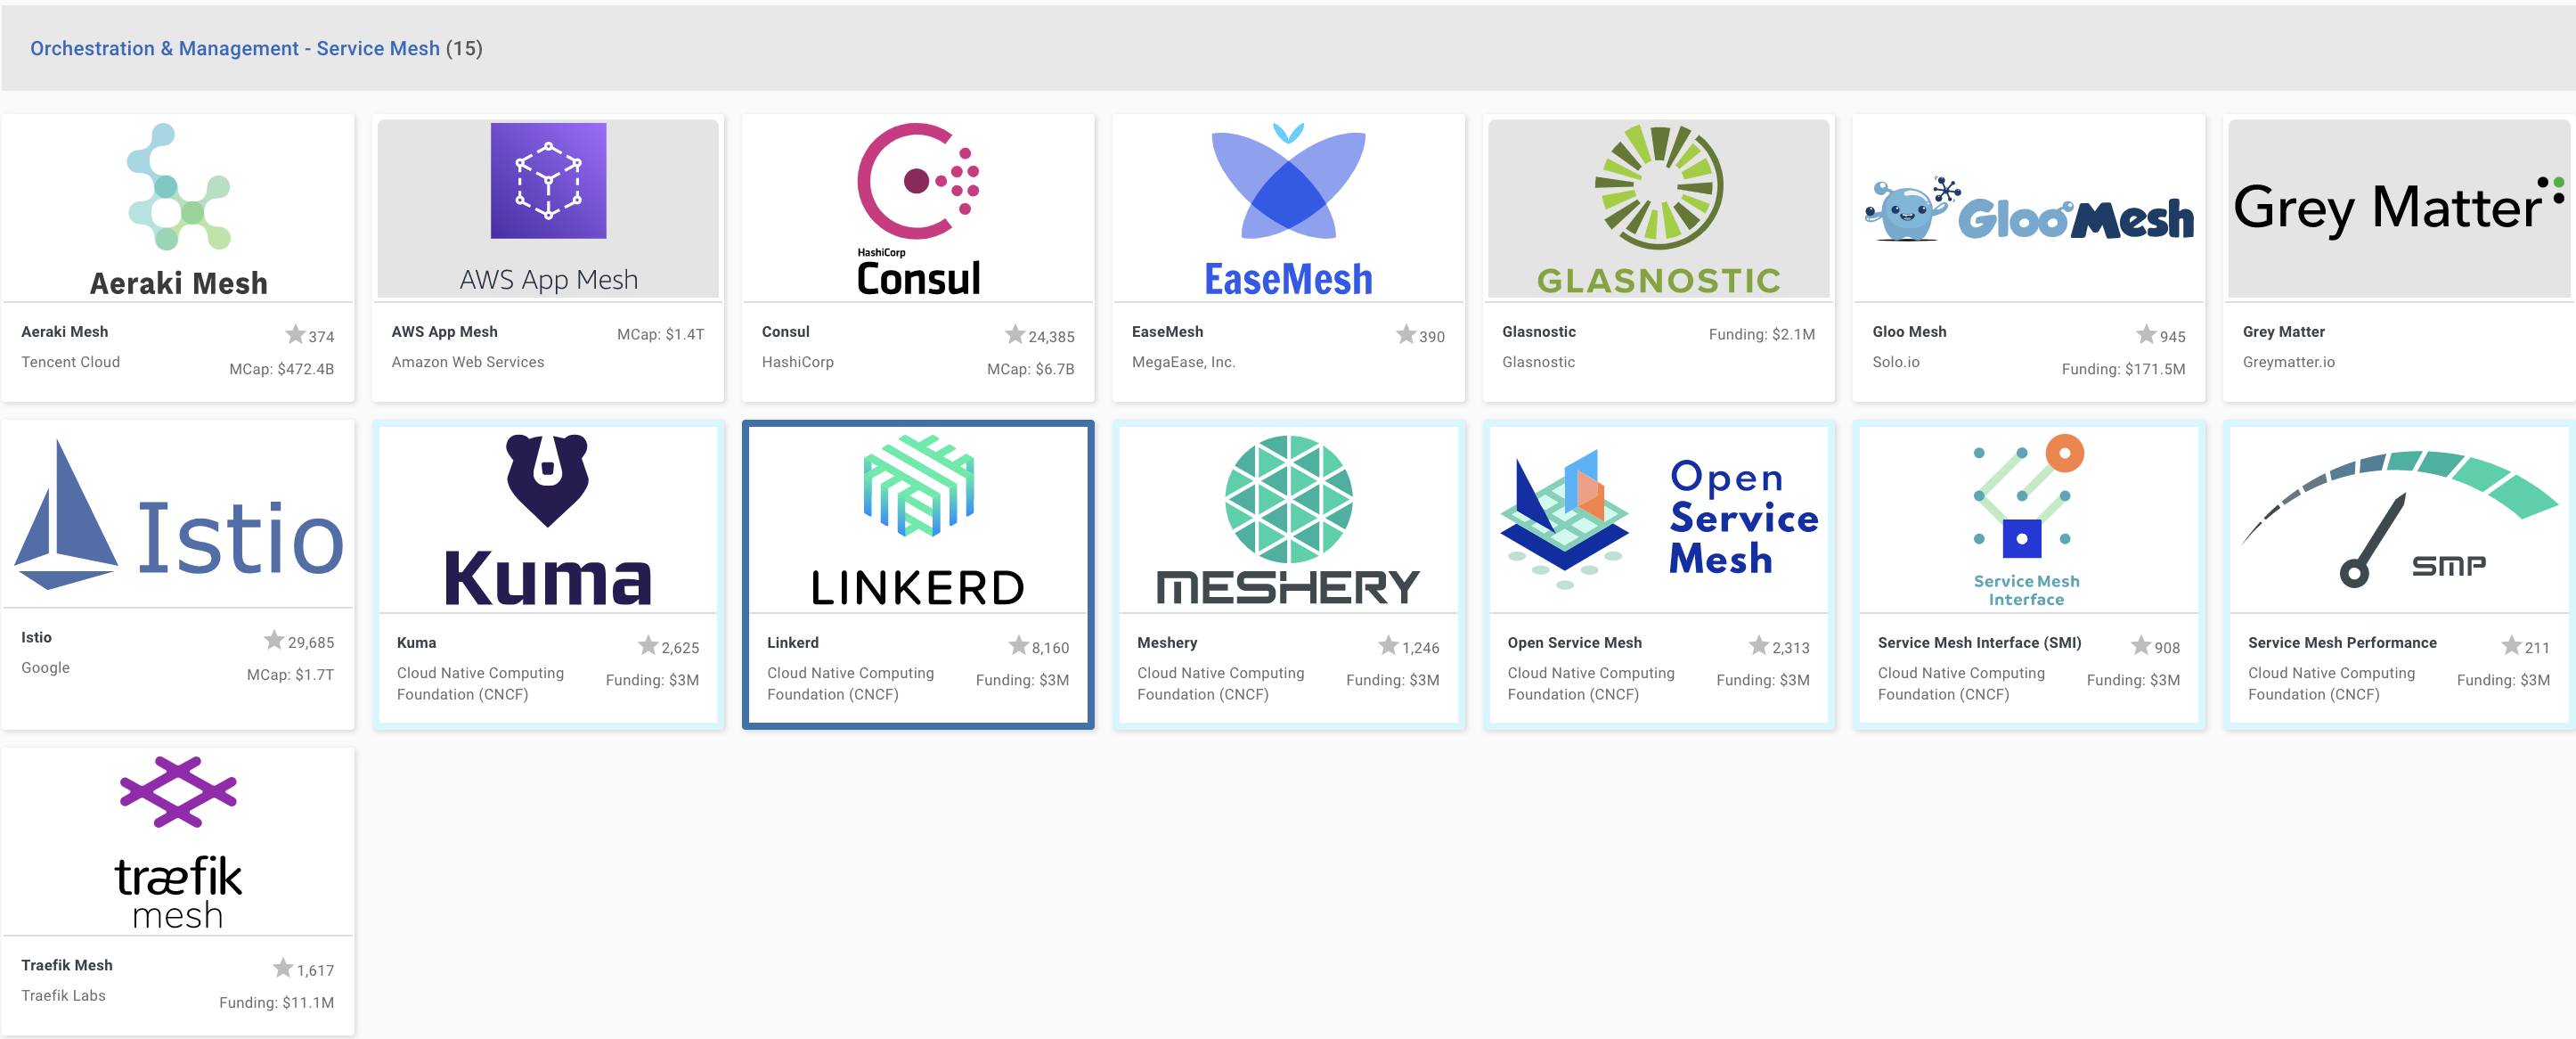
\includegraphics[width=0.9\linewidth]{3_systems_survey/figures/cncf-landscape-service-mesh}
    \caption[CNCF landscape of \gls{sm} technologies]{\gls{cncf} landscape of \gls{sm} technologies as of March 2022}
    \label{fig:cncf-landscape-sm}
\end{figure*}

\todo{Discuss this section, it was previously related work for system/lit. surveys.}

To justify a formal systematic survey we first evaluate the existing related work in the field. In \cref{sec:background:related-work:survey}, we discuss the singular secondary study that we identified before executing this system survey. We concluded, similarly to the authors of the paper, that there is a lack of academic literature in this field. Even though the work  from Li et al. \cite{service-mesh-survey} was concluded in 2019, the situation still prevails. This provides a sharp contrast with the amount of attention the field has received from the industry as it contains an abundance of blog posts and talks. The author of one of the most popular \gls{sm} systems even went as far to call it the \say{the world’s most over-hyped technology} \cite{service-mesh-manifesto}. Aside from the attention it has been getting, it has also been shown that \gls{sm} systems are becoming increasingly popular as indicated in surveys conducted by Red Hat \cite{rh-surve-2022} and the \gls{cncf} \cite{cncf-survey-2020}.

In addition to the attention of the industry, the field has seen many developments. New systems have emerged, and existing systems have evolved. With very recent developments  \cite{istio-merbridge, cilium-mesh} (less than two months old at the time of writing) paving the way for fundamentally different approaches, the field is as exciting as it gets.

This all results in a justification for conducting the survey, and that the timing of it manages to capture an interesting, evolutionary shift within the field.


\section{Survey Objectives}
\label{sec:survey:objectives}
% What are we trying to achieve in this survey
% - Bridge the gap between academia and industry
% - Gain insights into the current state-of-the-art-systems
% - Obtain knowledge about relative metrics and workloads 
% - ^> Is a stepping stone to the next chapter

% - Tie it all to the research question defined in the introduction

Before conducting a systematic systems survey, we first establish a set of objectives which we will try to achieve in this work. This allows us to structure the research and adjust its methodologies based on the objectives. The following list represents the formulated objectives.

\begin{enumerate}[label=\textbf{O\arabic*}, leftmargin=3\parindent]
    \item \textbf{Bridge the gap between academia and industry.}
    \label{obj:survey:1}
    
    In the previous section (\cref{sec:survey:introduction}), we identified that there is a large gap between interest from academia and the industry. We identified that there is a lack of formal publications in the field, whereas preliminary exploration showed that this is in sharp contrast to the interest as expressed from the industry. This leads to this first objective, which is to close this gap and provide formal research in this emerging field.
    
    \item \textbf{Gain insight into the current state-of-the-art \gls{sm} systems.}
    \label{obj:survey:2}
    
    The second objective of this survey is to gain a clear understanding of the field and the current state-of-the-art \gls{sm} systems. We want to identify the systems that currently exist and identify their defining properties and characteristics.

    \item \textbf{Obtain knowledge about relevant performance related intricacies.}
    \label{obj:survey:3}
    
    Finally, we want to identify and analyse the properties and components that capture the performance implications of these systems. By examining these systems in detail, and by taking a closer look at the design of these systems, we can hypothesize on the performance complications of design decisions. This is important for the later parts of our work so that we can analyse the experimental results and relate back to architectural differences uncovered.
    
\end{enumerate}

% - Tie it all to the research question defined in the introduction
% - Tie it to the general flow of the thesis as this provides a stepping stone to further chapters
The objectives and their respective order in which they are  presented are closely tied to the general flow of research conducted within this thesis. We first established the gap between industry and academia in our previous work and formulated this thesis around the idea to close this \ref{obj:survey:1}. Furthermore, we apply best practices by conducting a survey of the field. This helps us to understand the field and allows us to examine the current state-of-the-art systems in detail \ref{obj:survey:2}. The data synthesis of this survey allows us to establish a framework to compare the existing and future \gls{sm} systems which might emerge. The results of this will be used to provide the answer to the research question \ref{rq-1} during our analysis. Additionally, the survey and resulting framework allows us to determine relevant metrics and components to measure \ref{obj:survey:3}. This provides a stepping stone towards the following chapter, in which we design an instrument to compare the performance characteristics of these systems (\cref{chap:system-design}).
\section{Methodology}
\label{sec:survey:methodology}

% General intro of what is happening in this chapter
% - Systematic approach to a survey (reproducible)
% - Section structure
The following section covers the methodology that is used throughout the systematic systems review. The idea of the systematic approach is to make the results as presented in this chapter reproducible. This is done by extensively detailing the methodology used and explaining the decisions we had to take. We present the guidelines, data sources and steps taken to reach the dataset used in the data synthesis. 

The remainder of this section is structured as follows. First, in \cref{sec:survey:methodology:strategy} we identify and discuss methods and techniques commonly used in systems surveys. Secondly, in \cref{sec:survey:methodology:approach}, we combine the methods and techniques identified, and present the strategy that we used to approach this survey. Subsequently, we introduce the research protocol that we established to conduct the survey.




\subsection{Defining a Strategy}
\label{sec:survey:methodology:strategy}

% Introduction to strategy definition


There are many methods and techniques out there to find, select or synthesize the data for a survey. The methodology and technique used throughout such a survey ultimately dictates the form a survey takes on and influences the results it produces. It is important to identify, compare and choose such methods and techniques that fit the needs of our system-focussed survey. 

In this section, we will present the identified methods that we can use for a survey. For each method, we discuss their advantages and disadvantages and whether we will use them in some form within the survey.

\subsubsection{Unguided Techniques}
\label{sec:survey:methodology:strategy:unguided}

% Analysis of common survey methods
% - Unguided Methods
% - Unguided Search -> Initial dataset
% - Backward Snowballing -> Enhange datase


\textit{Unguided search} is the first technique that we have identified. This technique is commonly used to produce an initial dataset of relevant literature on the topic. This process requires the researcher to traverse various digital libraries equipped with relevant keywords to produce the dataset. Another commonly used technique that we have identified is \textit{backward snowballing}. This is another unguided method often used as a complementary technique to expand the dataset and is achieved by searching for related papers in the reference section. By combining these techniques, a researcher can create a literature review based on the generated dataset. However, both of the techniques are unguided, and therefore the process is not reproducible. Using such unguided techniques can result in entirely different datasets if the process is to be repeated by another researcher, and thus does not produce much scientific value. 

% Analysis of common survey methods
% - Guided Methods
% - SLR (Kitchenham) -> Planning, Conducting, Reporting
% - Petersen -> comparative analysis guidelines
\subsubsection{Systematic Approach}
\label{sec:survey:methodology:strategy:systematic}

% SLR
To prevent any form of bias to have an effect on the process and results of a survey, we have to establish and utilize a systematic approach. We have identified a state-of-the-art methodology which aims to create a systematic process which will be used to guide this survey. The works of Kitchenham and Charters \cite{Kitchenham2007} introduce a battle-tested and auditable set of guidelines for literature reviews aimed at software engineering researchers  with the goal of promoting reproducibility. The introduced \textit{\gls{slr}} methodology consists of three steps, planning the review, conducting the review and reporting the review. We decided to use these guidelines as a baseline for the survey, as it aligns with our goals and environment.

In addition to the guidelines introduced by the \gls{slr} methodology, we utilize the guidelines as introduced in the works of Petersen et al. \cite{Petersen2008, Petersen2015}. The authors introduce a set of guidelines and techniques which can be used to conduct a mapping study on a given topic. Among the guidelines and techniques, the authors introduce a method to perform comparative analysis. These guidelines and methods align with our needs and goals to compare \gls{sm} systems in the field as stated by the formulated research question \ref{rq-1}. 

% MLR method (Garousi)
% - MLR (Garousi) -> Inclusion of GL
\subsubsection{Inclusion of Grey Literature}
\label{sec:survey:methodology:strategy:gl}

% - Previous lit survey -> Lack of PL
% - 2019 Secondary survey -> Lack of PL
% - Most content from the industry is GL
One of the drawbacks of the \gls{slr} method is that it only concerns \gls{pl}, which consists of published peer-reviewed academic articles. In our previous work, in which we have conducted a systematic literature review on the \gls{k8s} ecosystem, we came to the conclusion that this field lacked published and peer-reviewed articles. Additionally, previous secondary studies on the field came to the same conclusion \cite{service-mesh-survey}. The lack of published (formal) literature in the field makes it impossible for us to conduct the research to an extent which satisfies our goals. This led us to explore additional forms of literature. \Gls{gl} is a form of literature that does not belong in the formal category, and can be in the form of blog posts, videos or white papers. Exploratory research has shown that inclusion of \gls{gl} can be beneficial to our research, as most of the literature is presented in such form by the industry.

% - Introduction to MLR
To maintain a systematic approach with the inclusion of \gls{gl}, we had to define or find additional guidelines that supported this requirement. We have identified the state-of-the-art method for conducting a survey which enabled the inclusion of \gls{gl}. The \gls{mlr} methodology as introduced by Garousi et al. \cite{Garousi2019} adapts and extends the \gls{slr} method from Kitchenham et al. so that it can include both forms of literature. 

% MLR checklist table
\begin{table*}[t]
\centering
\resizebox{\linewidth}{!}{ %< auto-adjusts font size to fill line
    \begin{tabular}{@{}lll@{}}
    \toprule
    \# & Question & Answer \\
    \midrule
    1 & Is the subject “complex” and not solvable by considering only the formal literature? & Yes \\
    2 & Is there a lack of volume or quality of evidence, or a lack of consensus of outcome measurement in the formal literature? & Yes \\
    3 & Is the contextual information important to the subject under study? & Yes \\
    4 & Is it the goal to validate or corroborate scientific outcomes with practical experiences? & Yes \\ 
    5 & Is it the goal to challenge assumptions or falsify results from practice using academic research or vice versa? & No \\ 
    6 & Would a synthesis of insights and evidence from the industrial and academic community be useful to one or even both communities? & Yes \\ 
    7 & Is there a large volume of practitioner sources indicating high practitioner interest in a topic? & Yes \\ 
    \bottomrule
    \end{tabular}
} %< \resizebox
\caption[Questionnaire to decide whether to include \gls{gl}. ]{Questionnaire from the works of Garoussi et al. \cite{Garousi2019}, which helps to decide whether to include \gls{gl} in a literature survey.}
\label{tab:mlr-checklist}
\end{table*}

% - MLR requriements checklist
Additionally, the authors have created a checklist which can be used to verify the need for inclusion of \gls{gl} within a survey. If one or more of the questions in the checklist is answered with a \say{yes}, it indicates that \gls{gl} can be beneficial to the survey. We answered the questions in the provided checklist and the results of this can be seen in \cref{tab:mlr-checklist}. These results reaffirmed our requirement for \gls{gl} throughout the survey and made us adapt the guidelines as described by the methodology.




\subsection{Our Approach to a Systematic Survey}
\label{sec:survey:methodology:approach}
%  Summarize entire approach and present figure that shows this
% - SLR Leeading
% - MLR -> inclusiong of GL
% - Petersen -> comparitive analysis

In the previous section (\cref{sec:survey:methodology:strategy}), we identified several methodologies and guidelines which we can use to conduct a survey. We explained why we have chosen some of these guidelines for our systems survey and how they could apply to our research goals. The resulting strategy can be seen in more detail in the form of a flow chart in  \cref{fig:survey-methodology}. This figure depicts two of the three stages in from the \gls{slr} methodology, namely the planning phase and the conducting phase. It also lists all the deliverables of this systems survey (\designref{D1} - \designref{D5}). 

Up to this point, we have discussed two steps of the planning phase. This first step of the planning phase \designref{P1}, consists of establishing a need for the survey, which we did in \cref{sec:survey:related-work}. Next, we established our goals \ref{g-1} - \ref{g-3} and research question \ref{rq-1} in \cref{sec:survey:goals} which relates to process \designref{P2}.




% Support findings based on some perspectives
\begin{figure}[!t]
    \centering
    
    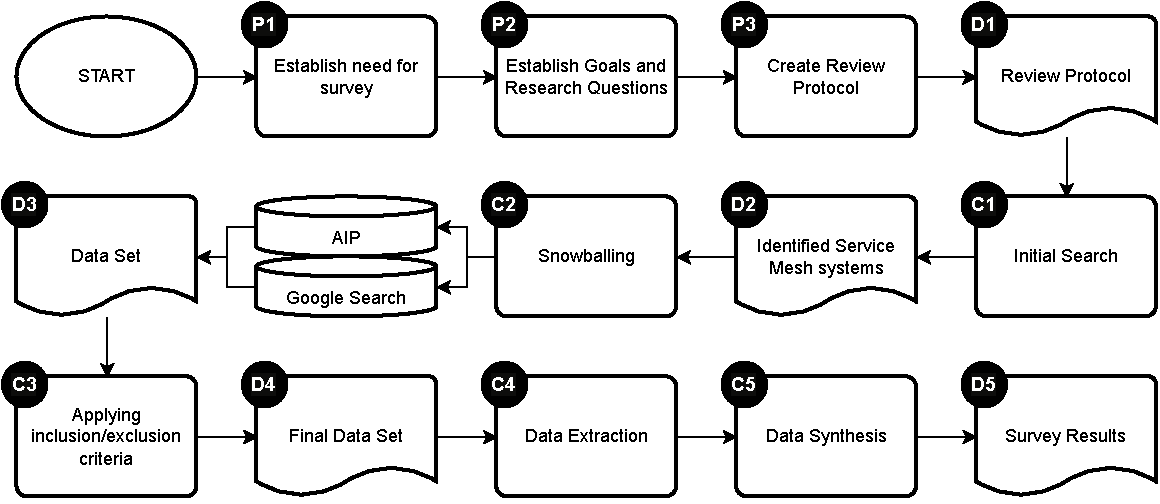
\includegraphics[width=\linewidth]{3_systems_survey/figures/survey-methodology}

    \caption{System Survey approach.}
    \label{fig:survey-methodology}
\end{figure}




% % SLR Plannign phase
% % 1. Investigate need (rel. work)
% % 2. Objective of this research
% % 3. Formulate RQ.
% \subsection{Planning}
% \label{sec:survey:methodology:planning}

% \todo{Fix planning section}

% In line with the guidelines as proposed in the \gls{slr} methodology, we first conducted a planning stage. During this stage we have analysed relevant work and the need for a review as discussed in \cref{sec:survey:related-work}. After this, we formulated the goal and related research question of this survey as seen in \cref{sec:survey:goals}. The goal of this systems survey is to uncover the existing \gls{sm} systems in the landscape and provide an overview of characteristics that they have. By creating a data synthesis of the literature that we are able to find on this topic, we can produce a general framework to contain these systems. This is a stepping stone for the research that is conducted in the later chapters, in which we examine and evaluate the characteristics and performance properties of these systems in more detail. 



% SLR - Review Protocol
\subsection{Review Protocol}
\label{sec:survey:methodology:review-protocol}

% Review protocol consists of
% - Background, the rationale for the survey -> Goals
% - Research Questions that we intend to answer


% PL & GL
% - Search Strategy
% - Selection Criteria
% - Selection Procedures
% - Data Extraction



The review protocol is a fundamental aspect of the \gls{slr} methodology, it specifies the methods used to conduct the systems review in this thesis. A pre-defined protocol is required to reduce the possibility of any bias. Establishing the review protocol is part of our approach as specified in \cref{fig:survey-methodology} and depicts the process \designref{P3}.

In the remainder of this section, we introduce the components that establish the research protocol. In \cref{sec:survey:methodology:review-protocol:search-strategy}, we introduce the search strategy which is used to search for the relevant literature. In \cref{sec:survey:methodology:review-protocol:selection-criteria}, we establish the selection criteria which are used to filter the dataset which we obtained through the research strategy. Finally, in \cref{sec:survey:methodology:review-protocol:data-extraction}, we describe the methods used to extract and synthesize the data.



\subsubsection{Search Strategy}
\label{sec:survey:methodology:review-protocol:search-strategy}
% - Data Sources
% - Queries

To create a reproducible data set, we have to establish a search strategy which we use to obtain literature on the topic. The search strategy differs based on the type of literature, where different requirements apply for \gls{pl} and \gls{gl}.


% Data sources
% - AIP
% - Digital Libraries (DBLP, Aminer, Semantic Scholar)
% - Only established, well respected conferences
The first component that makes up the search strategy is related to the data sources. The Atlarge  team\footnote{\url{https://atlarge-research.com/}} has identified several digital libraries which are well established and which contain the leading publications in the field of distributed systems. Additionally, years of experience in the field led to the creation of a list of established and well-respected conferences. This consolidated knowledge led to the development of a software instrument \gls{aip}. This instrument is used to generate the initial dataset of \gls{pl} for this survey and query it. To establish a dataset of \gls{gl} in this survey, we use Google Search to identify relevant literature.

The second component of the search strategy is related to the search technique. Since the goal of this survey to compare state-of-the-art \gls{sm} systems, we first have to identify said systems. To achieve that, we first conducted exploratory research in the field. To reduce bias in this process, we first used the single identified secondary study \cite{service-mesh-survey} to obtain an initial set of \gls{sm} systems. After this, we identified the \gls{sm} systems that were part of official \gls{cncf} projects\footnote{\url{https://landscape.cncf.io/card-mode?category=service-mesh&grouping=category}}, as they have proven to be an authoritative entity in the field as discussed in \cref{sec:background:cncf}. This list was then complemented by results obtained from \gls{gl} using generic search queries. 


The final component of the search strategy is related to the search queries that we use to establish the resulting dataset. To find and identify the current state-of-the-art \gls{sm} systems, we used generic terms as described above. After this, we utilized a snowballing method in which we based the search queries on the identified systems. The final list of search queries used can be seen in \cref{tab:search-queries}. Queries \textbf{Q1} and \textbf{Q2} represent the queries used to obtain and expand the list of identified \gls{sm} systems, while \textbf{Q3} indicates the system-specific queries that were used. 

\begin{table}[t]
\centering
% \resizebox{\linewidth}{!}{ %< auto-adjusts font size to fill line
    \begin{tabularx}{\linewidth}{lXl}
    \toprule
    \# & Query & Search Strategy \\
    
    % Initial Search Queries
    \midrule
    \textbf{Q1} & Service Mesh & Initial Search \\
    \textbf{Q2} & Service Mesh Implementation & Initial Search \\

    % Queries Based on identified SM systems
    \midrule
    \textbf{Q3} & \textit{Identified Service Mesh Implementation} & Snowballing  \\
    
    \bottomrule
    \end{tabularx}
% } %< \resizebox
\caption{Search queries established in the review protocol.}
\label{tab:search-queries}
\end{table}

% \begin{table}[t]
% \centering
% % \resizebox{\linewidth}{!}{ %< auto-adjusts font size to fill line
%     \begin{tabular}{@{}lll@{}}
%     \toprule
%     \# & Query & Search Strategy \\
    
%     % Initial Search Queries
%     \midrule
%     \textbf{Q1} & Service Mesh & Initial Search \\
%     \textbf{Q2} & Service Mesh Implementation & Initial Search \\

%     % Queries Based on identified SM systems
%     \midrule
%     \textbf{Q3} & \textit{Identified Service Mesh Implementation} & Snowballing  \\
    
%     \bottomrule
%     \end{tabular}
% % } %< \resizebox
% \caption{Search queries established in the review protocol.}
% \label{tab:search-queries}
% \end{table}



\subsubsection{Selection Criteria}
\label{sec:survey:methodology:review-protocol:selection-criteria}
% Seperate Criteria for PL and GL
% Introduce the checklist and how it works
% display PL and GL checklist
Since we have decided to also include \gls{gl} in our survey, we decided to establish two sets of selection criteria since they are vastly different in terms of content and medium. For both types of literature, we establish a checklist. In this checklist, we define the guidelines that we use to either include or exclude a data point. Guidelines prefixed with a checkmark (\cmark) symbol indicate a reason to include a publication in the research, whereas the cross (\xmark) symbol indicates a reason for exclusion. 

The following checklist (\cref{list:checklist:pl}) contains a set of selection criteria that applies to the \gls{pl} that is obtained through the search process. For this, we apply a set of generic criteria in order to 

In addition to the search queries, we used a filter to filter out any results before 2014 since that the initial release date of \gls{k8s} \cite{kubernetes-overview}. This limits the results based on the scope of this research, which provides a focus on \gls{sm} systems in the \gls{k8s} ecosystem.

\begin{itemize}
    \item[(\cmark)] Publications that are written in English.
    \item[(\cmark)] Publications introducing novel concepts.
    \item[(\cmark)] Publications that focus on architectural problems and solutions.
    \item[(\cmark)] Publications performing performance analysis studies.
    
    \item[(\xmark)] Publications before 2014. 
    \item[(\xmark)] Publications that do not have \gls{sm} systems as the primary subject in the research. 
    \item[(\xmark)] Secondary or tertiary studies regarding \gls{sm} systems.
    \item[(\xmark)] Publications that are not full-text (e.g., small snippets or as part of a demo).
    
    \label{list:checklist:pl}
\end{itemize}


The following checklist (\cref{list:checklist:gl}) contains a set of selection criteria that applies to the \gls{gl} that is obtained through the search process. For this form of literature we had to establish a set of rigorous guidelines since it can otherwise result in numerous data entries or lead to a biased set of results. 

\begin{itemize}
    \item[(\cmark)] Publications that are written in English.
    \item[(\cmark)] Publications introducing novel concepts.
    \item[(\cmark)] Publications originating from well established and known organizations (e.g. \gls{cncf}, Google, Red Hat, etc.).
    \item[(\cmark)] Publications that supply official vendor or platform documentation.
    \item[(\cmark)] Publications in the form of blog posts from organizations or authorities in the field.
    \item[(\cmark)] Publications in the form of videos from talks or conferences related to the field.
    \item[(\cmark)] Source code repositories of open-source \gls{sm} systems (e.g., a GitHub repository).
    
    \item[(\xmark)] Publications in which we cannot validate the authority of an author (e.g., anonymous posts, or posts by someone not established in the field). 
    \item[(\xmark)] Publications which do not provide any novelty for the survey (e.g., tutorials on the technologies). 
    \item[(\xmark)] Publications that are not full-text (e.g., small snippets, parts of a demo or short social media excerpts such as tweets).
    
    \label{list:checklist:gl}
\end{itemize}


\subsubsection{Data Extraction}
\label{sec:survey:methodology:review-protocol:data-extraction}
% What kind of information is relevant to us
% Compare systems
% Observability
% Resilience
% Proxy Characteristics
% Protocol Support
% Security
% Meta


Once we have established a final dataset by filtering the dataset based on the selection criteria, we can start the data synthesis process. To achieve this, we first have to establish a set of data extraction guidelines. These guidelines have to be in line with the goals which of this survey. Since we want to compare  state-of-the-art \gls{sm} systems, we have to identify the key characteristics and properties  of such systems. Through the preliminary research conducted on the field, we understand the fundamentals of a \gls{sm} system and have identified the challenges it tries to solve. With this in mind, we try to identify and synthesize the data based on key areas.


% Observability
% Resilience
% Proxy Characteristics
% Protocol Support
% Security
% Meta
First off, we try to compare these systems based on their architectural approach. With this take, we can identify and compare \gls{sm} systems based on their design decisions, such as their control and data plane components. Secondly, we take a functional approach to synthesize these systems. By identifying sets of functionality, we can evaluate and compare these systems on domain-specific functionalities such as their observability, security, or resiliency characteristics. Furthermore, we take a meta analytical approach to these systems. With this, we try to establish certain aspects such as the number of users the system has, the development activity on the project, whether a project is open-source or not and the maturity of the system.
\section{Results}
\label{sec:survey:results}

% General intro of what is happening in this chapter
% - Identified Service Mesh Systems
% - Identified requirements
% - Comparison Framework

In this section, we present the results from the systems survey as deliverable \designref{D5}. First, we present the identified \gls{sm} systems in \cref{sec:survey:results:sm-systems}. Furthermore, in \cref{sec:survey:results:sm-requirements} we introduce functional and non-functional requirements which we use to differentiate \gls{sm} systems. Finally, in \cref{sec:survey:results:sm-framework} we present a comparison framework for state-of-the-art \gls{sm} systems, in which we compare the identified systems.


% Identified SM systems
% - 12 Systems
% - Why we dont include managed istio services
\subsection{State-of-the-art Service Mesh Systems}
\label{sec:survey:results:sm-systems}

During the initial phase of the systems survey, we set out to identify existing \gls{sm} systems with our initial search strategy (\textbf{Q1} \& \textbf{Q2} in \cref{tab:search-queries}). During this phase, we identified 14 different \gls{sm} systems, which can be seen in \cref{tab:sm-implementations}, which represents deliverable \designref{D2}. By identifying these systems, we could run targeted queries on these them, which enabled us to dive deeper into their individual architectures.

% SM Implementations table
\begin{table*}[t]
\centering
\resizebox{\linewidth}{!}{ %< auto-adjusts font size to fill line
    \begin{tabular}{@{}lll@{}}
    \toprule
    ID & Service Mesh & Vendor Page \\
    
    % Included SM implementations
    \midrule
    \textbf{SM1}\label{sm1} & AWS App Meshh & \url{https://aws.amazon.com/app-mesh/} \\
    \textbf{SM2}\label{sm2} & Cilium & \url{https://cilium.io/} \\
    \textbf{SM3}\label{sm3} & Consul & \url{https://www.consul.io/} \\
    \textbf{SM4}\label{sm4} & Ease Mesh & \url{https://megaease.com/easemesh/} \\
    \textbf{SM5}\label{sm5} & Istio & \url{https://istio.io/} \\
    \textbf{SM6}\label{sm6} & Kuma & \url{https://kuma.io/} \\
    \textbf{SM7}\label{sm7} & Linkerd2 & \url{https://linkerd.io/} \\
    \textbf{SM8}\label{sm8} & Nginx Service Mesh & \url{https://www.nginx.com/products/nginx-service-mesh} \\
    \textbf{SM9}\label{sm9} & Open Service Mesh & \url{https://openservicemesh.io/} \\
    \textbf{SM10}\label{sm10} & Traefik Mesh & \url{https://traefik.io/traefik-mesh/} \\
    
    % Excluded SM implementations
    \midrule
    \textbf{-} & Alibaba Cloud Service Mesh & \url{https://www.alibabacloud.com/product/servicemesh} \\
    \textbf{-} & Aspen Mesh & \url{https://aspenmesh.io/} \\
    \textbf{-} & Citrix ADC & \url{https://www.citrix.com/nl-nl/products/citrix-adc/} \\
    \textbf{-} & Linkerd & \url{https://linkerd.io/} \\
    \bottomrule
    \end{tabular}
} %< \resizebox
\caption[Identified \gls{sm}.]{Identified \gls{sm} systems and their respective vendor pages. The \gls{sm} systems with an ID as indicated in the table, will be used and referred to throughout the rest of the system survey.}
\label{tab:sm-implementations}
\end{table*}

However, some systems in the list will be excluded from the rest of the work presented in this thesis. In particular, \textit{Alibaba Cloud Service Mesh},  \textit{Aspen Mesh}, \textit{Citrix ADC}, and \textit{Linkerd} are excluded. The first two systems are managed, closed-source service offerings of the popular \textit{Istio} \gls{sm}. The third system, has the option to utilize  \textit{Istio} to construct a \gls{sm}. We excluded these systems, as they provide no unique capabilities, are presented in the form of black box software and additionally has a financial cost attached to it. Finally, the last of the excluded systems mentioned, is superseded by \textit{Linkerd2} and is discontinued. 

% Identified SM systems
\subsection{Identified Requirements}
\label{sec:survey:results:sm-requirements}

To compare existing \gls{sm} systems, we have to introduce a set of requirements to compare them on. We do this in the form of \textit{Functional Requirements} and \textit{Non-Functional Requirements}. The former set of requirements describe the functions and characteristics of a system, such as the features and capabilities a specific system has. The latter, however, take a more general approach to describing the systems on its behaviour.

% Most important aspects of a service mesh
\subsubsection{Functional Requirements}
\label{sec:survey:results:sm-requirements:fr}

In this section, we introduce a list of six \textit{Functional Requirements} (\ref{fr-1} - \ref{fr-4}). We derived these requirements from the core functionalities of \gls{sm} systems. For each of the defined requirements, we provide a brief description of what the requirement entails and how we extract the information from the identified systems to measure this.


\begin{enumerate}[label=\textbf{FR\arabic*}, leftmargin=3\parindent]
    \item \textbf{Observability Capabilities}
    \label{fr-1}
    Indicates whether the system supports a wide variety of observability capabilities. Observability characteristics range from capturing metrics, to monitoring and tracing. To determine this, we have established a list of capabilities on which we compare these systems.
    
    \item \textbf{Security Capabilities}
    \label{fr-2}
    Indicates whether the system supports common security capabilities. To determine this, we first established a list of common security features, on which we compare the individual systems.
    
    \item \textbf{Resilience Capabilities}
    \label{fr-3}
    Indicates whether the system supports a wide variety of reliability characteristics. \Gls{sm} systems can improve the reliability of service-to-service communications in a system. To determine the capabilities of an individual system, we established a list of common reliability characteristics and compared the individual systems to these capabilities.
    
    \item \textbf{Support for Multiple Deployment Models}
    \label{fr-4}
    Indicates whether the system supports multiple deployment models. The most common scenario is to have a single cluster and a single service mesh. However, situations might exist where a topology consists of multiple clusters or multiple \glspl{sm} to provide for extra isolation, for example. We compare the identified systems to check for support on this characteristic.
\end{enumerate}


\subsubsection{Non-Functional Requirements}
\label{sec:survey:results:sm-requirements:nfr}

In this section, we introduce a list of six \textit{Non-Functional Requirements} (\ref{nfr-1} - \ref{nfr-5}). We established this list to provide for a general overview of the \gls{sm} systems. For each of the defined requirements, we provide a brief description of what the requirement entails and how we extract the information from the identified systems to measure this.



\begin{enumerate}[label=\textbf{NFR\arabic*}, leftmargin=3\parindent]
    \item \textbf{Application Protocol Support}
    \label{nfr-1}
    Service proxies can be aware of application level protocols to allow application level routing and rich metrics. This requirement indicates whether a \gls{sm} system supports a wide variety of application level protocols. To determine this, we established a list of common service-to-service protocols and also identified additional application level protocol support for each of the identified systems. The requirement is only fully satisfied if, in addition to the commonly listed protocols, it supports additional application level protocols.

    \item \textbf{Open-source}
    \label{nfr-2}
    Indicates whether a \gls{sm} system is available in the form of open-source software. To determine this, we identified source code repositories for the individual \gls{sm} systems if they existed.
    
    \item \textbf{Thoroughly Documented}
    \label{nfr-3}
    Indicates whether the system is extensively documented. This is determined by examining the vendor documentation on the system. The requirement is not satisfied if there is no vendor documentation partially satisfied if there is some form of vendor documentation, but not extensive or up to date, and fully satisfied if there is extensive and well-written documentation on the system.
    
    \item \textbf{Cloud Native Computing Foundation Project}
    \label{nfr-4}
    
    Indicates whether a \gls{sm} system is recognized as an official \gls{cncf} project and if so, which level of maturity it currently has. The \gls{cncf} defines three levels of maturity for each of its projects and imposes certain guidelines to achieve a new level of maturity \cite{cncf-project-graduation-criteria}. The projects and their levels ranging from \textit{sandbox} to \textit{incubating} to \textit{graduating} can be found on their website \footnote{\url{https://landscape.cncf.io/card-mode?category=service-mesh&grouping=category}} and can indicate the maturity of a project. The requirement is not satisfied if it is not a formal project, partially satisfied if it is in the \textit{sandbox} or \textit{incubating} stage, and fully satisfied if it is a \textit{graduated} project.


    \item \textbf{Community Recognition}
    \label{nfr-5}
    
    Indicates the recognition as per the community of users. We determine this by looking at various metrics and surveys regarding the usage of individual systems. For example, with open-source projects, we use community-related metrics such as GitHub stars. The requirement is partially satisfied if it has more than $10.000$ GitHub stars or more than 10 percent usage in production, according to the \gls{cncf} survey conducted in 2021 \cite{cncf-survey-2021}. To fully satisfy this requirement, the project needs more than $20.000$ GitHub stars or has more than 25 percent usage in production. 
\end{enumerate}



\subsection{Comparing Service Mesh Systems}
\label{sec:survey:results:comparison}

In this section, we present the results of the data synthesis based on the identified Functional and Non-Functional Requirements (\cref{sec:survey:results:sm-requirements:fr}, \cref{sec:survey:results:sm-requirements:nfr}). First, in \cref{sec:survey:results:comparison:proxy}, we compare the \gls{sm} systems on their service-to-service proxy. Secondly, in \cref{sec:survey:results:comparison:observability}, we compare the systems based on their observability capabilities. After that, in \cref{sec:survey:results:comparison:security}, we compare the systems on the most common security features. Following that, in \cref{sec:survey:results:comparison:resilience}, we evaluate the resiliency features of the systems. Finally, in \cref{sec:survey:results:comparison:nfr}, we show the obtained non-functional requirements regarding the systems. These results provide a stepping stone to the analysis in \cref{sec:survey:analysis}.

\subsubsection{Proxy Systems}
\label{sec:survey:results:comparison:proxy}
% Custom vs Common proxy
% Architectural Style
% Traffic Proxy

\begin{table*}[t]
\centering
\resizebox{\linewidth}{!}{ %< auto-adjusts font size to fill line
\begin{tabular}{ll|llcc}


\toprule

% HEADER 1
\multicolumn{2}{c|} {\textbf{Service Mesh}} &
\multicolumn{4}{c} {\textbf{Service Proxy Capbilities}}  \\

% HEADER 2
ID &
Name &
Service Proxy &
Proxy Architecture &
Proxy TCP &
Proxy UDP \\


\midrule


\textbf{SM1} &
AWS App Mesh  & 
Envoy & 
Per-Service & 
\cmark & 
\cmark \\


\textbf{SM2} &
Cilium  & 
Cilium (\gls{ebpf}) & 
In-Kernel & 
\cmark & 
\cmark \\


\textbf{SM3} &
Consul  & 
Envoy* & 
Per-Service & 
\cmark & 
\cmark \\


\textbf{SM4}&
Ease Mesh & 
Easegress & 
Per-Service & 
\cmark & 
\xmark \\


\textbf{SM5} &
Istio & 
Envoy & 
Per-Service & 
\cmark & 
\cmark \\


\textbf{SM6} &
Kuma & 
Envoy & 
Per-Service & 
\cmark & 
\cmark \\


\textbf{SM7} &
Linkerd2 & 
Linkerd2 Proxy & 
Per-Service & 
\cmark & 
\xmark \\


\textbf{SM8} &
Nginx Service Mesh & 
NGINX Plus & 
Per-Service & 
\cmark & 
\cmark \\


\textbf{SM9} &
Open Service Mesh  & 
Envoy & 
Per-Service & 
\cmark & 
\cmark \\


\textbf{SM10} &
Traefik Mesh &
Traefik Proxy & 
Per-Node & 
\cmark & 
\cmark \\


\bottomrule
\end{tabular}

} %< \resizebox
\caption
[Comparing the proxy capabilities of service mesh systems.]
{Comparing the proxy capabilities of identified service mesh systems. \\

\textit{Service Proxy} indicates the type of proxy component used, as this is considered an implementation detail of the service mesh architecture (see background \cref{sec:background:service-mesh}). \\
\textit{Proxy Architecture} refers to the manner in which the proxy is introduced within the system (see \cref{sec:survey:analysis:architectures}). \\
\textit{Proxy TCP} and \textit{Proxy UDP} support features indicate whether the \textit{Service Proxy} can proxy this type of traffic or whether it just forwards the type of traffic. 

\cmark: Indicates that the feature is supported. \\
\xmark: Indicates that the feature is no supported. \\
*: Can be interchanged for other service proxies.
}
\label{tab:result-proxy}
\end{table*}







% \begin{table*}[t]
% \centering
% \resizebox{\linewidth}{!}{ %< auto-adjusts font size to fill line
% \begin{tabular}{l|llll}
% \toprule
% Service Mesh       & Service Proxy  & Proxy Architecture & Proxy TCP & Proxy UDP \\
% \midrule
% AWS App Mesh       & Envoy          & Per-Service        & Yes       & Yes       \\
% Cilium             & Cilium eBPF    & Kernel (eBPF)      & Yes       & Yes       \\
% Consul             & Envoy*         & Per-Service        & Yes       & Yes       \\
% Ease Mesh          & Easegress      & Per-Service        & Yes       & No        \\
% Istio              & Envoy          & Per-Service        & Yes       & Yes       \\
% Kuma               & Envoy          & Per-Service        & Yes       & Yes       \\
% Linkerd2           & Linkerd2 Proxy & Per-Service        & Yes       & No        \\
% Nginx Service Mesh & NGINX Plus     & Per-Service        & Yes       & Yes       \\
% Open Service Mesh  & Envoy          & Per-Service        & Yes       & Yes       \\
% Traefik Mesh       & Treafik Proxy  & Per-Node           & Yes       & Yes       \\
% \bottomrule
% \end{tabular}

% } %< \resizebox
% \caption
% [Comparing the service-to-service proxy mechanisms of service mesh systems.]
% {Comparing the service-to-service proxy mechanisms of service mesh systems.

% *: Can be interchanged for other service proxies.
% }
% \label{tab:result-proxy}
% \end{table*}



First off, we compared the service-to-service proxy mechanisms of the identified \gls{sm} systems. At the core of a \gls{sm} system lies the service-proxy, it serves as the data-plane of the system and has a huge impact on the flow of traffic. The result of this comparison can be seen in \cref{tab:result-proxy}. While some \gls{sm} systems have their own custom service proxy, such as \textit{Linkerd2}, others utilize popular open-source proxy implementations such as \textit{Envoy}. Not all service proxies work and behave the same, the architecture of a proxy has a major impact on the traffic flow of a \gls{sm} system. During this survey, we have identified three different types of proxy architectures. First off, we identified a per-service proxy, such as used by most of the identified service proxies. This means that every service gets its own service proxy, and thus the number of proxies linearly scales with the number of services. The second architectural style identified is a per-node proxy, this is used by the \textit{Traefik Proxy}. This means that there is a single proxy per node, and that all services running on a node use that same proxy. The third and final architectural style identified also makes use of a single proxy per node but manages the traffic in the kernel space using \gls{ebpf}. Furthermore, we identified for each of the proxy systems if it was able to proxy TCP and UDP traffic. Being able to proxy TCP and/or UDP traffic means that the system will intercept any traffic of that type, and proxy it to the appropriate destinations. \Gls{sm} systems without UDP traffic proxy support can still have UDP traffic in their system, however, with the traffic not passing through the proxy it will provide none of the features that a \gls{sm} traditionally provides such as observability, security and resilience.


\subsubsection{Observability}
\label{sec:survey:results:comparison:observability}
% Metics system -> Nearly all prometheus
% Monitoring system -> Nearly all grafana
% Tracinf Support -> Jaeger > Zipkin > Open Standard
% Additional Dashboard -> Some have, e.g. custom topology inspection

\begin{table*}[t]
\centering
\resizebox{\linewidth}{!}{ %< auto-adjusts font size to fill line
\begin{tabular}{l|lllll}
\toprule
Service Mesh       & Metrics        & Monitoring     & Tracing                     & Dashboard \\
\midrule
AWS App Mesh       & AWS CloudWatch & AWS CloudWatch & AWS CloudWatch              & AWS X-Ray \\
Cilium             & Prometheus     & Grafana        & Jaeger, Open Telemetry      & Hubble    \\
Consul             & Prometheus     & Grafana        & Jaeger, Zipkin, OpenTracing & Consul UI \\
Ease Mesh          & Ease Monitor   & Ease Monitor   & OpenTracing                 & No        \\
Istio              & Prometheus     & Grafana        & Jaeger, Zipkin              & Kiali     \\
Kuma               & Prometheus     & Grafana        & Jaeger, Zipkin              & Yes       \\
Linkerd2           & Prometheus     & Grafana        & Open Telemetry              & Yes       \\
Nginx Service Mesh & Prometheus     & Grafana        & Jaeger                      & No        \\
Open Service Mesh  & Prometheus     & Grafana        & Jaeger                      & No        \\
Traefik Mesh       & Prometheus     & Grafana        & Jaeger                      & No        \\
\bottomrule
\end{tabular}
} %< \resizebox
\caption{Comparing the observability capabilities of identified service mesh systems.}
\label{tab:result-observability}
\end{table*}



Observability is a key feature and reason to use a \gls{sm}. The proxying of service-to-service communications allows systems to implement per-service metrics such as latencies, request volumes and error rates. We compared the identified \gls{sm} systems on key observability requirements, and the results of that can be seen in \cref{tab:result-observability}. First off, we identified the way in which the systems report metrics. Most of the identified systems made use of \textit{Prometheus}, a popular open-source time-series metric aggregator.  Furthermore, we compared the ways the systems enabled monitoring. Once again, \gls{sm} implementations resort to the same solution, this time in the form of \textit{Grafana}, a monitoring and observability platform. Tracing support, on the other hand, showed more variability. Most of the identified systems support \textit{Jaeger}, an open-source distributed tracing system. \textit{Zipkin} was another popular system with support, and some systems even supported open standards such as \textit{Open Telemetry}, allowing for any tracing system that supports that standard. Some \gls{sm} systems come with a bundled dashboard or have popular open-source extensions which enable this. These dashboards provide additional domain specific insights, such as provide graph tools to visualize the service mesh traffic topology. 

\subsubsection{Security}
\label{sec:survey:results:comparison:security}
% All services support MTLS (except Traefik)
% All services support S2S Authz (except Traefik)

\begin{table*}[t]
\centering
% \resizebox{\linewidth}{!}{ %< auto-adjusts font size to fill line

\begin{tabular}{ll|cc}


\toprule

% HEADER 1
\multicolumn{2}{c|} {\textbf{Service Mesh}} &
\multicolumn{2}{c} {\textbf{Security Capbilities}}  \\

% HEADER 2
ID &
Name &
Mutual TLS &
S2S Auth. Policies \\


\midrule


\textbf{SM1} &
AWS App Mesh  & 
\cmark  &
\cmark  \\

\textbf{SM2} &
Cilium  & 
\cmark  & 
\cmark \\


\textbf{SM3} &
Consul  & 
\cmark  & 
\cmark   \\


\textbf{SM4}&
Ease Mesh & 
\cmark  & 
\cmark \\


\textbf{SM5} &
Istio & 
\cmark  & 
\cmark   \\


\textbf{SM6} &
Kuma & 
\cmark  & 
\cmark   \\


\textbf{SM7} &
Linkerd2 & 
\cmark  & 
\cmark \\


\textbf{SM8} &
Nginx Service Mesh & 
\cmark & 
\cmark \\


\textbf{SM9} &
Open Service Mesh  & 
\cmark  & 
\cmark \\


\textbf{SM10} &
Traefik Mesh &
\xmark  & 
\xmark \\


\bottomrule
\end{tabular}
% } %< \resizebox

\caption[Comparing service mesh security capabilities]
{Comparing the security capabilities of identified service mesh systems.

\textit{Mutual TLS} indicates if the \gls{sm} system supports TLS authentications, which enables encrypted communications between service proxies. \\
\textit{S2S Auth. Policies} (Service-to-service authorization policies) indicate whether the \gls{sm} system supports advanced  authorization policies which enables the operator to grant or deny permissions to services to communicate with given entities (such as other services). \\

\cmark: Indicates that the feature is supported. \\
\xmark:  Indicates that the feature is no supported. }
\label{tab:result-security}
\end{table*}



Additional security is a feature that a \gls{sm} can provide. We compared the identified systems on the most common security characteristics a \gls{sm} can provide. The result of this can be seen in \cref{tab:result-security}. First, we identified if a \gls{sm} system can provide mutual TLS with little to no additional effort. This means that any service-to-service traffic is then encrypted and potential intruders in a network cannot inspect or intercept that traffic. All the systems, except \textit{Traefik Mesh}, support automatic mutual TLS encryption. Additionally, we compared the service-to-service authorization capabilities of these systems. This enables fine-grained control of access between services and users. Once again, all the systems, except \textit{Traefik Mesh}, have some form of authorization policies.

\subsubsection{Resilience}
\label{sec:survey:results:comparison:resilience}


\begin{table*}[t]
\centering
\resizebox{\linewidth}{!}{ %< auto-adjusts font size to fill line
\begin{tabular}{ll|cccccc}


\toprule

% HEADER 1
\multicolumn{2}{c|} {\textbf{Service Mesh}} &
\multicolumn{6}{c} {\textbf{Resiliency Capbilities}}  \\

% HEADER 2
ID &
Name &
Retry Funcionality &
Timeout Settings &
Rate Limiting &
Circuit Breaking &
Fault Injection &
Delay Injection \\


\midrule

\textbf{SM1} &
AWS App Mesh  & 
\cmark &
\cmark &
\xmark &
\cmark &
\xmark &
\xmark \\


\textbf{SM2} &
Cilium  & 
\cmark &
\cmark &
\cmark &
\cmark &
\cmark &
\cmark \\


\textbf{SM3} &
Consul  & 
\cmark &
\cmark &
\cmark &
\cmark &
\xmark &
\cmark\\


\textbf{SM4}&
Ease Mesh & 
\cmark &
\cmark &
\cmark &
\cmark &
\xmark  &
\xmark  \\


\textbf{SM5} &
Istio & 
\cmark &
\cmark &
\cmark &
\cmark &
\cmark &
\cmark \\


\textbf{SM6} &
Kuma & 
\cmark &
\cmark &
\cmark &
\cmark &
\cmark &
\cmark\\


\textbf{SM7} &
Linkerd2 & 
\cmark &
\cmark &
\xmark &
\xmark &
\cmark &
\xmark \\


\textbf{SM8} &
Nginx Service Mesh & 
\cmark &
\cmark &
\cmark &
\cmark &
\xmark &
\xmark \\


\textbf{SM9} &
Open Service Mesh  & 
\xmark &
\xmark &
\xmark &
\xmark &
\xmark &
\xmark \\


\textbf{SM10} &
Traefik Mesh &
\cmark &
\cmark &
\cmark &
\cmark &
\xmark &
\xmark \\

\bottomrule
\end{tabular}
} %< \resizebox
\caption[Comparing service mesh resiliency capabilities]
{Comparing the resiliency capabilities of identified service mesh systems.

\cmark: Indicates that the feature is supported. \\
\xmark:  Indicates that the feature is no supported. }
\label{tab:result-resilience}
\end{table*}



Managing applications in distributed systems is a complex task and can often lead to unwanted failures. Networks, compute nodes or applications can fail and cascade throughout the workload. To mitigate or resolve these problems, we can introduce distributed systems best practices to improve the resilience. In \cref{tab:result-resilience}, we compared the resiliency functionalities of identified \gls{sm} systems. First off, we compared the systems on the ability to retry failed service requests. Most of the systems, except \textit{Open Service Mesh}, supported this functionality. Furthermore, we identified and compared the systems on their ability to allow and tweak the timeout settings of service-to-service communications. Furthermore, we identified and compared the systems on their ability to support rate limiting. Rate-limiting in this context refers to the ability to tweak maximum request per second settings on a per-user or per-service level. Next, we evaluated the systems on their ability to support circuit breaking, this allows the system to prevent cascading failures by for example preventing traffic to reach an individual service instance if this instance fails requests too frequently. Finally, we compared the systems on their support for fault injections and delayed fault injections. These features allow the user to evaluate the resiliency of their applications by injecting faulty requests and timeouts, and can catch bugs in service integrations.


\subsubsection{Application-Level Protocol Support}
\label{sec:survey:results:comparison:protocols}
% Most are application aware of the same protocols
% Some support HTTP3
% Some have additional protocol support


\begin{table*}[t]
\centering
\resizebox{\linewidth}{!}{ %< auto-adjusts font size to fill line
\begin{tabular}{ll|ccccccc}

\toprule

% HEADER 1
\multicolumn{2}{c|} {\textbf{Service Mesh}} &
\multicolumn{7}{c} {\textbf{Protocol Support}}  \\

% HEADER 2
ID &
Name &
HTTP1.1 &
HTTP2 &
HTTP3 &
Websockets &
gRPC &
TLS &
Additional Protocols \\

\midrule

\textbf{SM1} &
AWS App Mesh  & 
\cmark &
\cmark &
\cmark &
\cmark &
\cmark &
\cmark &
- \\


\textbf{SM2} &
Cilium  & 
\cmark &
\cmark &
\cmark &
\cmark &
\cmark &
\cmark &
Kafka \\


\textbf{SM3} &
Consul  & 
\cmark &
\cmark &
\cmark &
\cmark &
\cmark &
\cmark &
- \\


\textbf{SM4}&
Ease Mesh & 
\cmark &
\cmark &
\xmark &
\cmark &
\xmark &
\cmark &
MQTT \\


\textbf{SM5} &
Istio & 
\cmark &
\cmark &
\cmark &
\cmark &
\cmark &
\cmark &
Mongo, Redis, MySQL  \\


\textbf{SM6} &
Kuma & 
\cmark &
\cmark &
\cmark &
\cmark &
\cmark &
\cmark &
Kafka \\


\textbf{SM7} &
Linkerd2 & 
\cmark &
\cmark &
\xmark &
\cmark &
\cmark &
\cmark &
- \\


\textbf{SM8} &
Nginx Service Mesh & 
\cmark &
\cmark &
\xmark &
\cmark &
\cmark &
\cmark &
- \\


\textbf{SM9} &
Open Service Mesh  & 
\cmark &
\cmark &
\cmark &
\cmark &
\cmark &
\cmark &
- \\


\textbf{SM10} &
Traefik Mesh &
\cmark &
\cmark &
\cmark &
\cmark &
\cmark &
\cmark &
- \\

\bottomrule
\end{tabular}
} %< \resizebox
\caption[Comparing service mesh proxy protocol support capabilities]
{Comparing the application level protocol support of identified service mesh systems.

\cmark: Indicates that the feature is supported. \\
\xmark: Indicates that the feature is no supported. }
\label{tab:result-protocols}
\end{table*}




Not all service proxies are the same, some are built to be very minimal and fast, whereas others try to provide as much functionality as possible. We evaluated the identified \gls{sm} systems on their application level protocol support, as shown in \cref{tab:result-protocols}. To have advanced proxy capabilities such as routing and rich metrics, the protocol must be determined and understood. All the systems support the most common service-to-service protocols in the form of \textit{HTTP/1.1} \textit{HTTP/2.0} and \gls{grpc}. This means that the user of such system can see the HTTP status codes in the metrics or route the traffic based on the HTTP headers present. Additionally, all the identified systems support web sockets and TLS encryption. Some systems have support for the newer \textit{HTTP/3.0} protocol, however, for all the identified systems that support this, the feature is in beta and bound to change. Finally, we identified some systems that support additional application level protocols. 



\subsubsection{Non-Functional Requirements}
\label{sec:survey:results:comparison:nfr}

\begin{table*}[t]
\centering
\resizebox{\linewidth}{!}{ %< auto-adjusts font size to fill line
\begin{tabular}{ll|lllllllll}


\toprule

% HEADER 1
\multicolumn{2}{c|} {\textbf{Service Mesh}} &
\multicolumn{8}{c} {\textbf{Non-functional Attributes}}  \\

% HEADER 2
ID &
Name &
Launched   & 
Initiator &
\makecell{CNCF \\ Project} & 
OSS & 
\makecell{GitHub \\ Stars} & 
Version & 
Licence & 
Lang. \\
\midrule


\textbf{SM1} &
AWS App Mesh  & 
27/03/2019 &
Amazon  & 
\xmark & 
\xmark & 
- & 
- & 
- & 
- \\


\textbf{SM2} &
Cilium  & 
02/12/2021 & 
Isovalent & 
\circleH & 
\cmark & 
11149 & 
Beta & 
Apache & 
Go \\


\textbf{SM3} &
Consul  & 
26/06/2018 &
Hashicorp &
\xmark & 
\cmark & 
24423 &
1.11.4 &
Mozilla &
Go \\


\textbf{SM4}&
Ease Mesh & 
01/02/2021 &
MegaEase &
\xmark &
\cmark & 
396 &
1.2.0 &
Apache &
Java \\

\textbf{SM5} &
Istio &
19/11/2016 &
Google &
\xmark &
\cmark & 
29770 &
1.13.2 &
Apache &
Go \\


\textbf{SM6} &
Kuma & 
13/03/2019 &
Kong &
\circleE &
\cmark & 
2637 &
1.5.0 &
Apache &
Go \\


\textbf{SM7} &
Linkerd2 & 
05/12/2017 &
Buoyant &
\circleF &
\cmark & 
8207 &
1.7.5 &
Apache &
Go \\


\textbf{SM8} &
Nginx Service Mesh & 
12/10/2020 &
Nginx &
\xmark &
\xmark & 
- &
1.4.0 &
- &
- \\


\textbf{SM9} &
Open Service Mesh  & 
13/12/2019 &
Microsoft &
\circleE &
\cmark & 
2343 &
1.0 &
Apache &
Go \\


\textbf{SM10} &
Traefik Mesh &
03/03/2019 &
Traefik &
\xmark &
\cmark & 
1622 &
1.4.5 &
Apache &
Go \\


\bottomrule
\end{tabular}
} %< \resizebox
\caption[Comparing the non-functional attributes of service mesh systems]{Comparing the non-functional attributes of identified service mesh systems.

Circles in the table indicate the level of maturity for \gls{cncf} projects: \\
\circleE: Sandbox \\
\circleH: Incubating \\
\circleF: Graduated \\
\cmark: Indicates that the attribute conforms. \\
\xmark: Indicates that the attribute does not conform. }
\label{tab:result-nfa}
\end{table*}

Finally, we identified several non-functional requirements of each of the identified service mesh systems. The result of this can be seen in \cref{tab:result-nfa}. We identified the launch date of a \gls{sm} system by either the first official vendor blog post or commit in an open-source repository, if available. Furthermore, we identified which company or initiated the project, this can give an indication on the amount of backing a project can get. Next up, we determined if the \gls{sm} system is part of any formal\gls{cncf} project, and if so at which stage it currently is, this can indicate a level of maturity. We also determined if the system is available as open-source software. If the project was open-source, we were able to determine other requirements, such as the current version number, licence and main programming language used as well as the amount of stars the project has which can give an insight in community recognition. Every identified open-source system had a remote repository on GitHub, for which we extracted the previously mentioned attributed through their public API\footnote{\url{https://docs.github.com/en/rest}}.

\section{Analysis of System Survey}
\label{sec:survey:analysis}


In the previous section (\cref{sec:survey:results}), we conducted a data synthesis process on the data we obtained during the systems survey. This process resulted in domain-specific characteristics of identified service mesh systems. In this section, we continue with the data and analyse and discuss notable differences we discovered during the data synthesis process.

The remainder of this section is structured as follows. In \cref{sec:survey:analysis:sm-framework}, we provide a qualitative comparison of the service mesh systems and present several key findings from the obtained data. Thereafter, in \cref{sec:survey:analysis:architectures}, we dive into the different architectures and how they can relate to the observed behaviour. Finally, in \cref{sec:survey:analysis:conclusion}, we provide an answer to \ref{rq-1} and conclude the systems survey.


\subsection{Qualitative Comparison of Service Mesh Systems}
\label{sec:survey:analysis:sm-framework}
% Display resulting framework
% Explain per FR, NFR how it is measured
% Introduction to how it might relate to architecture
% Observations
% - Architecture -> Most Per-Service
% - Traefik Mesh -> No MTLS
% - Three systems fully hit all functional requirements
% - Linkerd2 -> Different Focus

In \cref{tab:result-comparison}, we present a qualitative evaluation of state-of-the-art service mesh systems. In this comparison, we present the architectural style the service proxy uses and map the identified requirements and their level of satisfaction (\cref{sec:survey:results:sm-requirements} to each individual system. 

\begin{table}[!t]

\centering
\resizebox{\linewidth}{!}{ %< auto-adjusts font size to fill line
\begin{tabular}{c|cc|cccc|ccccc}
\toprule

% HEADER 1
\multicolumn{1}{c|}{} &
\multicolumn{2}{c|}{\textbf{Data Plane}} &
\multicolumn{4}{c|}{\textbf{Functional Requirements}} &
\multicolumn{5}{c}{\textbf{Non-Functional Requirements}}  \\

% HEADER 2
\multicolumn{1}{c|}{\textbf{Service Mesh}} &
\multicolumn{1}{c}{\textbf{Service Proxy}}  &
\multicolumn{1}{c|}{\textbf{Proxy Arch.}}  &
\multicolumn{1}{c}{\ref{fr-1}}  &
\multicolumn{1}{c}{\ref{fr-2}}  &
\multicolumn{1}{c}{\ref{fr-3}}  &
\multicolumn{1}{c|}{\ref{fr-4}} &

\multicolumn{1}{c}{\ref{nfr-1}} &
\multicolumn{1}{c}{\ref{nfr-2}} &
\multicolumn{1}{c}{\ref{nfr-3}} &
\multicolumn{1}{c}{\ref{nfr-4}} &
\multicolumn{1}{c}{\ref{nfr-5}} \\

\midrule
% CONTENT

AWS App Mesh
& Envoy         % Service Proxy
& Per-Service   % Proxy Architecture
& \circleF      % FR1 Observability
& \circleF      % FR2 Security
& \circleH      % FR3 Resilience
& \circleF      % FR4 Additional Deployment Models

& \circleH      % NFR1 Application Level Protocol Aware
& \circleE      % NFR2 Open-Source
& \circleF      % NFR3 Documentation
& \circleE      % NFR4 CNCF Level
& \circleE      % NFR5 Commmunity Recognition
\\

Cilium
& Cilium eBPF   % Service Proxy
& In Kernel     % Proxy Architecture
& \circleF      % FR1 Observability
& \circleF      % FR2 Security
& \circleF      % FR3 Resilience
& \circleF      % FR4 Additional Deployment Models

& \circleF      % NFR1 Application Level Protocol Aware
& \circleF      % NFR2 Open-Source
& \circleH      % NFR3 Documentation
& \circleH      % NFR4 CNCF Level
& \circleH      % NFR5 Commmunity Recognition
\\

Consul
& Envoy         % Service Proxy
& Per-Service   % Proxy Architecture
& \circleF      % FR1 Observability
& \circleF      % FR2 Security
& \circleH      % FR3 Resilience
& \circleF      % FR4 Additional Deployment Models

& \circleH      % NFR1 Application Level Protocol Aware
& \circleF      % NFR2 Open-Source
& \circleF      % NFR3 Documentation
& \circleE      % NFR4 CNCF Level
& \circleH      % NFR5 Commmunity Recognition
\\

Ease Mesh
& EaseGress     % Service Proxy
& Per-Service   % Proxy Architecture
& \circleF      % FR1 Observability
& \circleE      % FR2 Security
& \circleH      % FR3 Resilience
& \circleE      % FR4 Additional Deployment Models

& \circleH      % NFR1 Application Level Protocol Aware
& \circleF      % NFR2 Open-Source
& \circleE      % NFR3 Documentation
& \circleE      % NFR4 CNCF Level
& \circleE      % NFR5 Commmunity Recognition
\\

Istio
& Envoy         % Service Proxy
& Per-Service   % Proxy Architecture
& \circleF      % FR1 Observability
& \circleF      % FR2 Security
& \circleF      % FR3 Resilience
& \circleF      % FR4 Additional Deployment Models

& \circleF      % NFR1 Application Level Protocol Aware
& \circleF      % NFR2 Open-Source
& \circleF      % NFR3 Documentation
& \circleE      % NFR4 CNCF Level
& \circleF      % NFR5 Commmunity Recognition
\\

Kuma
& Envoy         % Service Proxy
& Per-Service   % Proxy Architecture
& \circleF      % FR1 Observability
& \circleF      % FR2 Security
& \circleF      % FR3 Resilience
& \circleF      % FR4 Additional Deployment Models

& \circleF      % NFR1 Application Level Protocol Aware
& \circleF      % NFR2 Open-Source
& \circleF      % NFR3 Documentation
& \circleH      % NFR4 CNCF Level
& \circleE      % NFR5 Commmunity Recognition
\\

Linkerd2
& Linkerd2 Proxy% Service Proxy
& Per-Service   % Proxy Architecture
& \circleF      % FR1 Observability
& \circleF      % FR2 Security
& \circleH      % FR3 Resilience
& \circleF      % FR4 Additional Deployment Models

& \circleH      % NFR1 Application Level Protocol Aware
& \circleF      % NFR2 Open-Source
& \circleF      % NFR3 Documentation
& \circleF      % NFR4 CNCF Level
& \circleF      % NFR5 Commmunity Recognition
\\

Nginx Service Mesh
& NGINX Plus    % Service Proxy
& Per-Service   % Proxy Architecture
& \circleF      % FR1 Observability
& \circleF      % FR2 Security
& \circleH      % FR3 Resilience
& \circleE      % FR4 Additional Deployment Models

& \circleH      % NFR1 Application Level Protocol Aware
& \circleE      % NFR2 Open-Source
& \circleH      % NFR3 Documentation
& \circleE      % NFR4 CNCF Level
& \circleE      % NFR5 Commmunity Recognition
\\

Open Service Mesh
& Envoy         % Service Proxy
& Per-Service   % Proxy Architecture
& \circleF      % FR1 Observability
& \circleF      % FR2 Security
& \circleE      % FR3 Resilience
& \circleE      % FR4 Additional Deployment Models

& \circleH      % NFR1 Application Level Protocol Aware
& \circleF      % NFR2 Open-Source
& \circleH      % NFR3 Documentation
& \circleH      % NFR4 CNCF Level
& \circleE      % NFR5 Commmunity Recognition
\\

Traefik Mesh
& Traefik Proxy % Service Proxy
& Per-Node      % Proxy Architecture
& \circleF      % FR1 Observability
& \circleE      % FR2 Security
& \circleH      % FR3 Resilience
& \circleE      % FR4 Additional Deployment Models

& \circleH      % NFR1 Application Level Protocol Aware
& \circleF      % NFR2 Open-Source
& \circleH      % NFR3 Documentation
& \circleE      % NFR4 CNCF Level
& \circleE      % NFR5 Commmunity Recognition
\\
\bottomrule
\end{tabular}
} %< \resizebox

\caption[Qualitative comparison between state-of-the-art \gls{sm} systems.]{Qualitative comparison between state-of-the-art \gls{sm} systems. \\
There are three different symbols in the table, each of them represents how well a requirement is satisfied. \circleF: Fully Satisfied, \circleE: Not Satisfied, \circleH: Partially Satisfied.}
\label{tab:result-comparison}

\end{table}

We now present a list of the most interesting findings we obtained:

\begin{enumerate}[label=\textbf{F\arabic*}, leftmargin=3\parindent]
    \item \textbf{Most of the identified \gls{sm} systems share a similar data plane architecture.}
    \label{f-1}
    % Most use a per-service proxy
    % Most use envoy
    
    The first finding from the obtained data is that most of the systems use a similar architecture for the data plane of the \gls{sm}. Out of the ten identified \gls{sm} implementations, eight used a per-service proxy architecture. Furthermore, out of those eight using a per-service proxy architecture, half of them used the same service proxy implementation in the form of \textit{Envoy}, an open-source general purpose proxy.
    
    \item \textbf{Per-node data plane architecture prevents support for common security features.}
    \label{f-2}
    % Traefik uses per-node
    % Is the only one that does not support the security requirements
    
    The second finding is that only a single identified system used a service proxy architecture, where the service proxy was implemented on a per-node granularity. \textit{Traefik Mesh} is the identified service mesh that used such an architecture, and most notably it was the only implementation that did not support any of the security capabilities listed (\ref{fr-2}). In particular, it does not support automatic mutual TLS encryption between services, a killer feature to enhance the security in any environment. To further elaborate on this, we dive deeper into the characteristics of data plane architectures in the next section (\cref{sec:survey:analysis:architectures}).

    \item \textbf{Most identified systems do not support all functional requirements.}
    \label{f-3}
    % 3/10 implementations support all requirements
    % Cilium, Istio and Kuma
    % Cilium -> Network focus
    % Istio -> Feature focus + Mature + Complex
    % Kuma -> Feature focus, Extensibility, Support for different environments
    
    The third finding is that out of all ten identified service mesh systems, just three systems fully satisfy all the functional requirements (\ref{fr-1}-\ref{fr-4}), namely, \textit{Cilium}, \textit{Istio} and \textit{Kuma}. This finding can be explained by taking a closer look at the maturity levels and the goals that the individual \gls{sm} implementations have. The three identified services that achieve all functional requirements are mature projects or heavily emphasize their feature set and extensibility. \textit{Istio} is the most mature platform, with large backing and is the most used \gls{sm} implementation out of all identified systems according to the \gls{cncf} survey conducted in 2021 \cite{cncf-survey-2021}. It also supports the most features and therefore hits all the functional requirements. \textit{Kuma} on the other hand, is a much smaller project. However, its focus lies on having a broad feature set with lots of extensibility options as well, thus achieving all functional requirements as well. \textit{Cilium} on the other hand, is a new entry in the \gls{sm} landscape (as can be seen by the release date in the list of non-functional attributes (\cref{tab:result-nfa}). However, this story also does not paint the entirety of the picture as it builds upon the \textit{Cilium} networking solution, a mature networking solution that already facilitates most of the functional requirements listed.
    

    \item \textbf{Maturity does not translate to support of requirements.}
    \label{f-4}
    % Linkerd2 Does not hit all requirements
    % Different project focus
    % - Simple
    % - Fast
    % - Tailored proxy, less features
    
    A fourth finding is that maturity does not necessarily translate to the support of functional and non-functional requirements. This refers to \textit{Linkerd2} in particular, which does not  not fully satisfy the resiliency requirements \ref{fr-3} and also lacking in the additional application level protocol support \ref{nfr-1}. Despite its maturity, large-scale usage in production environments \cite{cncf-survey-2021}, and graduated \gls{cncf} project status, the system seems to be lacking in features. This, however, can be attributed to the goals of the project. Whereas \textit{Istio} has the most features of any system, it is also dubbed as a complex system. \textit{Linkerd2}, however, aims to optimize for simplicity and speed. Instead of using a generic proxy with numerous features and capabilities, such as \textit{Envoy} or \textit{NGINX}, it uses a custom proxy specifically tailored to the service mesh, optimizing for simplicity, security, and performance \cite{linkerd-no-envoy}.
    
    \item \textbf{Lack of additional layer 7 protocol support.}
    \label{f-5}
    % 4/10 systems support 'additional' layer 7 protocols
    % Why it is useful
    % External project (Aeraki) -> Tries to solve this
    
    A fifth finding is that just a few of the identified systems support additional application level protocols (\ref{nfr-1}). Since \gls{sm} systems can greatly benefit from additional application level support from its service proxies, it can be a promising area. It can enable application level aware traffic management, rich metric collection or can lead to advanced authorization policies. \textit{Cilium} and \textit{Kuma} for example, provide support for the Apache Kafka protocol and therefore can target specific messages when dealing with events of the platform.  Although we did identify only a few implementations that provided support for this, we did identify an external project in the \gls{cncf} landscape that tries to enable this. \textit{Aeraki}\footnote{\url{https://www.aeraki.net/}}, attempts to close this gap by creating an extensible platform that enables layer 7 support for many protocols such as \textit{Redis}, \textit{Kafka} and \textit{ZooKeeper}. This project, however, only provides support for \textit{Istio} and therefore currently does not support any other \gls{sm} implementation.
    
    \item \textbf{New technologies enable additional data plane architectures.}
    \label{f-6}
    % Single sm uses kernel based proxy (Cilium)
    % - Does not have linear dependency on proxy/service
    % - Relatively new techonology
    
    A final finding is that only a single project uses a kernel-based proxy. \textit{Cilium} uses a kernel-based proxy approach by utilizing \gls{ebpf} applications to implement the service proxy. Together with \textit{Traefik proxy}, it is the only \gls{sm} that does not use a per-service based data plane architecture. We can attribute this finding to the fact that \gls{ebpf} is a relatively new technology, and that the \textit{Cilium} networking project has been banking on that technology before extending its networking solution to include the properties of a service mesh in late 2021 \cite{cilium-mesh}. Although this is a fairly new approach, it has been adopted by one of the leading \gls{k8s} service providers in the form of \textit{Google Kubernetes Engine} \cite{google-cilium-ebpf}. Furthermore, other \gls{sm} systems also experiment with \gls{ebpf} technology to improve upon existing functionalities and support new features \cite{istio-merbridge, nginx-service-mesh-arch}. 
\end{enumerate}


% The first observation we can make from the obtained data is that most of the systems use a data plane with a per-service proxy. However, some \gls{sm} systems use a different approach, such as \textit{Traefik Mesh}, which uses a per-node proxy and \textit{Cilium}, which uses a kernel-based proxy. This can be attributed to the fact that half of the implementations use \textit{Envoy} as proxy, which is an open-source proxy. 

% The second observation that we can make is that \textit{Traefik Mesh} does not support any of the security capabilities listed (\ref{fr-2}). Notably, it does not support automatic mutual TLS encryption between services, a killer feature to enhance the security in any environment. This result, however, is unsurprising if we relate it to the first observation. Due to its per-node proxy, all service-to-service communications travel first from a service to the proxy in a potentially unencrypted state. This allows for potential attackers to intercept this, and thus to create a zero-trust environment application developers have to implement mutual TLS connections manually.

% The third observation is that there are three systems that fully satisfy all the functional requirements (\ref{fr-1}-\ref{fr-4}), namely, \textit{Cilium}, \textit{Istio} and \textit{Kuma}. The first of those systems has a heavy focus on networking and features, as it originates as a networking solution and transcended into the service mesh space since December 2021 \cite{cilium-ebpf-mesh}. The second of those systems can be considered the most mature \gls{sm} system, which sees the most amount of production use according to the \gls{cncf} 2021 survey \cite{cncf-survey-2021} and has enterprise backing. Kuma, on the other hand, is a project with much smaller backing and usage, however it has a focus on extensibility and features, even allowing the system in non-\gls{k8s} or vm-based environments. 

% A fourth observation is that \textit{Linkerd2} does not hit all the functional requirements as it does not fully satisfy the resiliency requirements \ref{fr-3} and also lacking in the additional application level protocol support \ref{nfr-1}. Despite its maturity, large-scale usage in production environments and graduated \gls{cncf} project status, the system seems to be lacking in features. This, however, can be attributed to the goals of the project. Whereas \textit{Istio} has the most features of any system, it is also dubbed as a complex system. \textit{Linkerd2}, however, aims to optimize for simplicity and speed. Instead of using a generic proxy with numerous features and capabilities, such as \textit{Envoy} or \textit{NGINX}, it uses a custom proxy specifically tailored to the service mesh, optimizing for simplicity, security and speed \cite{linkerd-no-envoy}.

% A fifth observation is that additional application level protocol support \ref{nfr-1} exists, however, not many systems have support for it out of the box. Since \gls{sm} systems can greatly benefit from application aware proxies, it can be a promising area. It can enable application level aware traffic management, rich metric collection or can lead to advanced authorization policies. Some proxies like \textit{Cilium} and \textit{Kuma} provide support for protocols such as \textit{Kafka}, in which they can target specific messages. Another project in the \gls{cncf} landscape under the name of \textit{Aeraki} \footnote{\url{https://www.aeraki.net/}}, attempts to close this gap by creating an extensible platform that enables layer 7 support for many protocols such as \textit{Redis}, \textit{Kafka} and \textit{ZooKeeper}. This project, however, only provides support for \textit{Istio} and therefore currently does not support any other \gls{sm} implementation.

% A final observation is that only a single project uses a kernel-based proxy. \textit{Cilium} uses a kernel-based proxy approach by utilizing \gls{ebpf} technology. Together with \textit{Traefik proxy}, it is the only \gls{sm} that does not use a per-service based data plane architecture. The reason for this is that \gls{ebpf} the technology is relatively new, and \textit{Cilium} has been banking on that technology before extending its networking solution to include the properties of a service mesh \cite{cilium-mesh}. Although this is a fairly new concept, it has been adopted by one of the leading \gls{k8s} service provider in the form of \textit{Google Kubernetes Engine} \cite{google-cilium-ebpf}. Furthermore, it is also used for a bleeding edge \textit{Istio} feature \cite{istio-merbridge} and in certain \textit{NGINX Service Mesh} beta features \cite{nginx-service-mesh-arch}.


\subsection{Analysis of Common Service Mesh Architectures}
\label{sec:survey:analysis:architectures}
% Introduce section
% Per-Service Arch
% Per-Node Arch
% Kernel

In this section, we analyse the identified \gls{sm} architectures in more detail. For every identified architecture, we present a reference topology and discuss the advantages and disadvantages one such implementation has. First, in \cref{sec:survey:analysis:architectures:per-service}, we discuss the most common identified approach, a \gls{sm} using a per-service proxy. Next, in \cref{sec:survey:analysis:architectures:per-node}, we discuss architectures leveraging a per-node proxy. Finally, in \cref{sec:survey:analysis:architectures:ebpf}, we discuss architectures using a kernel-based \gls{ebpf} approach.


\subsubsection{Per-Service Proxy}
\label{sec:survey:analysis:architectures:per-service}
% - Simplest architecture
% - Overhead, many proxies
% - Resource Usage
% - Latency / Hops

During the systems survey, we identified ten different \gls{sm} systems. Out of those ten systems, eight of those shared similar architectural characteristics. For all of these systems, we identified that the mesh network was established by introducing a proxy for every individual software service present. This architectural style is so common within the \gls{k8s} ecosystem, that the pattern is often referred to as the \textit{sidecar pattern}.


In \cref{fig:sm-arch-per-service}, we present a reference architecture of this design pattern for service meshes in a \gls{k8s} cluster. This shows the data path of a packet throughout its lifespan in a system that implements this architecture. To explain the data path of a packet, we first introduce the individual components depicted, as most of them are present in the other architectures as well. 

\begin{figure}[!t]
    \centering
    
    \scalebox{.8}{
    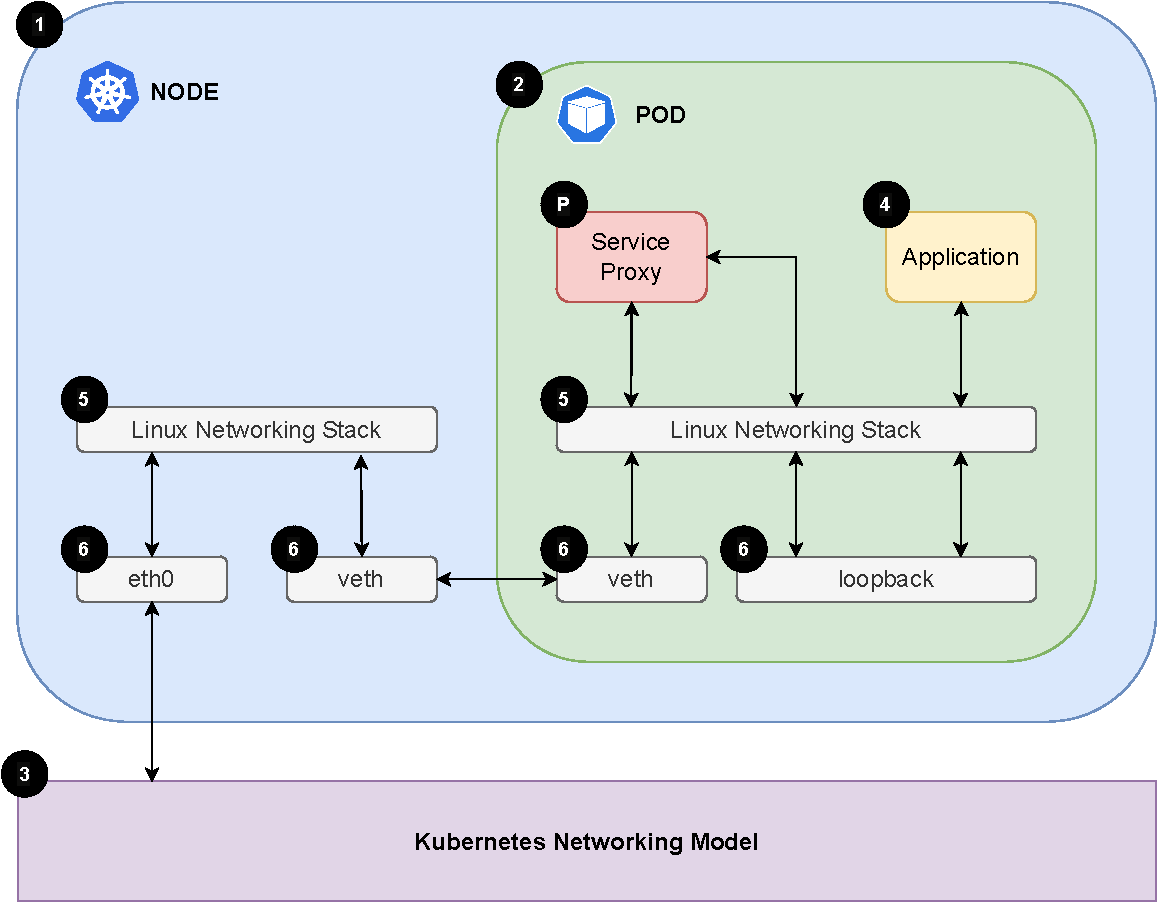
\includegraphics[width=\linewidth]{3_systems_survey/figures/sm-arch-per-service.pdf}
    }

    \caption[Per-service proxy plane architecture.]{The data path of a per-service data plane.}
    \label{fig:sm-arch-per-service}
\end{figure}

% Basic components introduction
First off, we have the node (\designref{1}), this represents a worker machine in \gls{k8s}, which can run workloads. Next up, we have a \gls{pod} (\designref{1}), this is the smallest unit of deployment within \gls{k8s} and consists of one or more application containers. The last \gls{k8s} related concept is the Kubernetes Networking Model (\designref{3}) \cite{kubernetes-cluster-networking}, which can be implemented in various ways, but has as goal to connect the nodes and pods within the cluster. Within the \gls{pod}, lives the actual application (\designref{4}), which can for example be a web server. The \textit{Linux Network Stack} (\designref{5}) is abstracted in this design as one single component, but consists of routing and filtering tables used to manage packets within the system. An important note, is that both the node and the \gls{pod} implement a separate networking stack, which isolates the pod network from the host network through network namespaces \cite{man-network-namespaces}. The traffic flows to physical and virtual network interfaces (\designref{6}) connected through one another, to reach its destination. Note that in actual deployments, more complex models are often present, such as bridge networks to support multiple pod networks or tunnel interfaces to create overlay networks, for instance. However, for this example, the added complexity does not help to illustrate the architectural differences at hand.


% Explain datapath
With the basic components of the reference architecture explained, we can take a closer look at the data path of a service request. Whenever a request to a service has been made that lives within the application pod (\designref{4}) a packet first enters the node. The inbound packet enters through the network interface (\designref{6}), has to pass through the kernel's networking stack (\designref{5}) to reach the \gls{pod}'s network namespace. After this, the traffic will reach the service proxy (\designref{P}) because it is configured to intercept all network traffic inside the pod. From there onwards, it has to travel through a loopback interface to finally reach the application. Replies from the application will traverse a similar, but inverse, data path.

% Advantages/Disadvantages
One of the advantages of such an architecture is that you can have fine-grained control over the traffic, as it is intercepted the moment it enters the namespace of the \gls{pod}. This characteristic allows the security features discussed during this systems review (\ref{fr-2}), and can for example enable encrypted connections between all traffic leaving a \gls{pod}. Furthermore, the \textit{sidecar pattern} allows for a very generic implementation, and does not require much if any modifications from the user's perspective. This enables a user-friendly user experience, while also allowing support for general purpose proxies such as \textit{Envoy} or \textit{HAProxy}. These advantages, make it so that this is the most common architectural approach identified. A disadvantage, however, is that this design introduces additional overhead. First off, it introduces an overhead in system resources, as there now is a network proxy for every software service. Furthermore, it introduces additional latency for the traffic, as for every service request, the packets travel through the proxy twice (ingress/egress).


\subsubsection{Per-Node Proxy}
\label{sec:survey:analysis:architectures:per-node}
% - Less overhead and hops
% - No MTLS

Another identified \gls{sm} architecture makes use of the per-node proxy. This architectural style is used by a single identified \gls{sm} system, \textit{Traefik Mesh}. We present this form of \gls{sm} architecture in \cref{fig:sm-arch-per-node}. Although many of the components in this system are similar and previously explained in \cref{sec:survey:analysis:architectures:per-service}, some differences change several characteristics drastically.

\begin{figure}[!t]
    \centering
    
    \scalebox{.8}{
    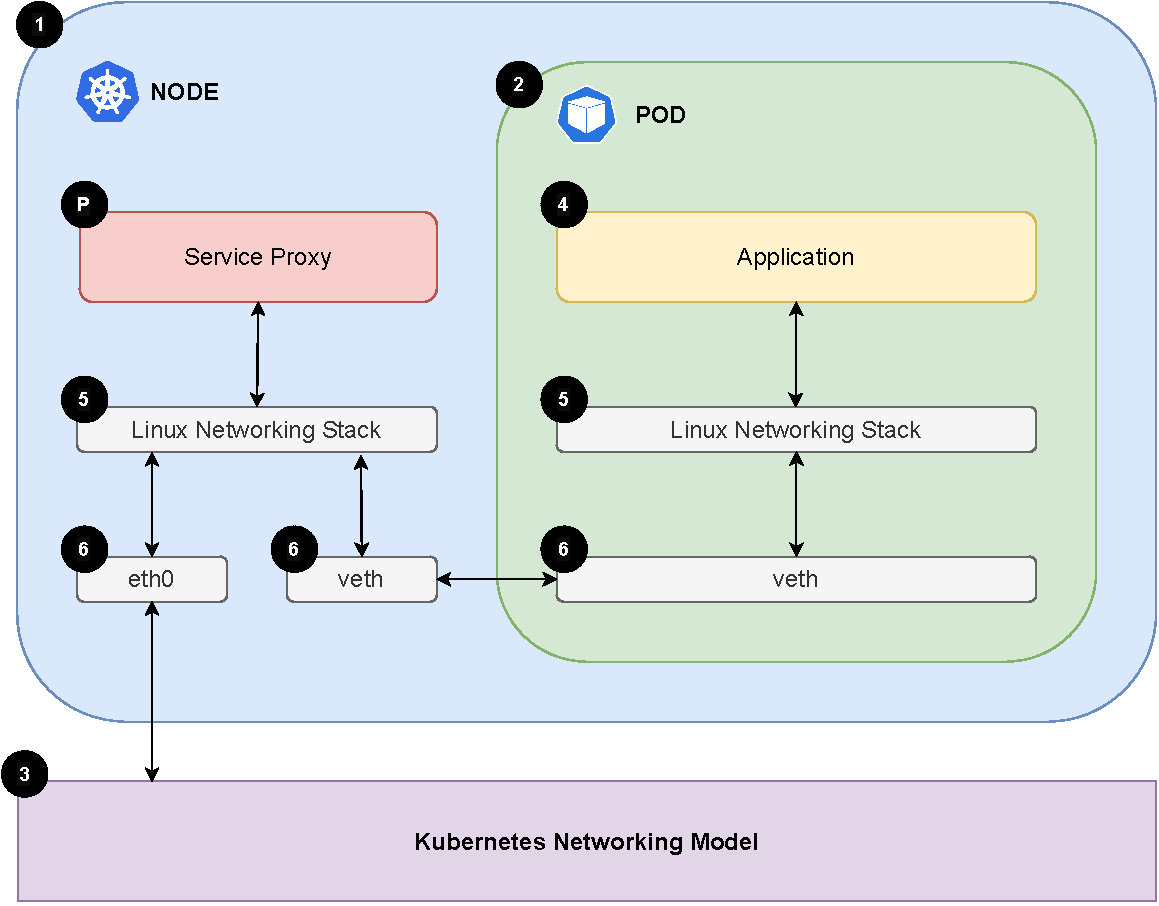
\includegraphics[width=\linewidth]{3_systems_survey/figures/sm-arch-per-node.pdf}
    }
    
    \caption[Per-node proxy plane architecture.]{The data path of a per-node data plane.}
    \label{fig:sm-arch-per-node}
\end{figure}

The most significant difference compared to the per-service architectural style is that service proxy (\designref{P}) is now not embedded within the \gls{pod} but lives within the node, thus makes use of the host network namespace. The reason for this is that this architectural style tries to limit the additional overheads caused by the introduces proxies of a \gls{sm}. This style of service proxies results in a single proxy per node, and thus does not scale linearly with the number of services on a node. This leads to the advantage that it consumes less system resources in the form of CPU cycles and memory. An additional benefit of this approach is that the traffic in the data path now has to traverse the proxy once in a service-to-service request. This halves the amount of service proxy hops compared to the previous solution. 

However, this architectural pattern comes at a cost. Since the traffic is not passing through the service proxies from within the pod, traffic enters the host network in a potentially compromised state. To elaborate this, the per-service approach allowed the traffic between proxies to be automatically encrypted using a mutual TLS connection, a characteristic evaluated during the system's review (\ref{fr-2}). This is, however, not possible as the data path outside the \glspl{pod} is not fully controlled and therefore has to be implemented manually. A downside is that when this is ignored, service-to-service data flows unencrypted through the node and therefore breaches well established security best practices such as the notion of zero trust networks \cite{zero-trust-network}.




\subsubsection{eBPF Proxy}
\label{sec:survey:analysis:architectures:ebpf}
% - New area
% - Faster, less hops
% - Potential security risks?
% -- Programmable Sandbox in kernel space

The last of the identified \gls{sm} architectures uses a vastly different approach. The approach used by \textit{Cilium} uses \gls{ebpf} to establish a mesh network between the services. What started out as a \gls{k8s} networking solution and evolved to become a fully fledged \gls{sm} implementation \cite{cilium-mesh}. 

% Shortened data path
In \cref{fig:sm-arch-ebpf}, we present a simplified data path of a \gls{sm} implemented using \textit{Cilium}.  Many of the components are shared with the other architectures and are explained in \cref{sec:survey:analysis:architectures:per-service}. However, compared to the other identified architectures, the data path as depicted here is much shorter. This is because the routing and proxying is done in the kernel through \gls{ebpf} (\designref{P}). 

% Explain EBPF
To explain the shortened data path, we first briefly have to introduce the technology powering it. \gls{ebpf} is a Linux Kernel technology that allows users to run sandboxed programs in the operating system kernel \cite{ebpf}. Furthermore, it is event-driven and allows these programs to execute on certain hooks. This is used throughout \textit{Cilium} to implement the observability, security and networking functionalities of the \gls{sm}. \gls{ebpf} allows for hooks throughout the entire lifecycle of a network packet. This combined with the programmable sandbox environments allows it to replace the role of service proxies in the other architectural styles. Since the \gls{ebpf} programs are aware of the \gls{k8s} endpoints and services, packets can be routed straight from the kernel, enabling a much more direct route.

% Advantages/Disadvantages
This architectural style has several advantages compared to the previously introduced per-service and per-node architectures. First, it has potential to decrease latency in its data path. It does this by not requiring additional hops in service-to-service communications. Additionally, it allows for greater programmability of the mesh network, as certain programs can be compiled and then run in a sandboxed environment. However, it also can have some disadvantages. First off, the technology and this implementation of it in particular is fairly new, even in a beta phase at the time of writing. This means that the \gls{sm} implementation could be unstable and not suitable for production usage. Furthermore, using user programs in kernel space could introduce potential security risks. 


\begin{figure}[!t]
    \centering
    
    \scalebox{.8}{
    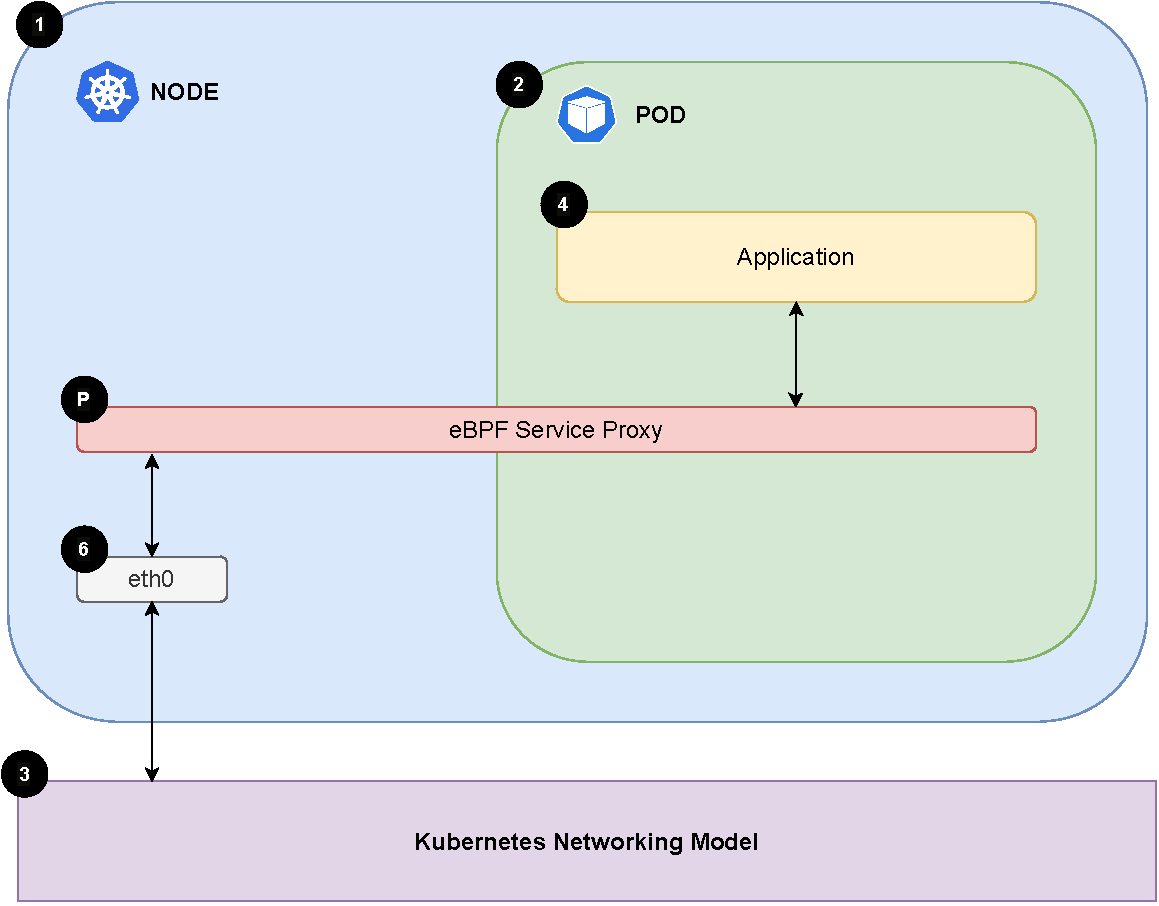
\includegraphics[width=\linewidth]{3_systems_survey/figures/sm-arch-ebpf.pdf}
    }
    
    \caption[\Gls{ebpf}-based data plane architecture.]{The data path of an \gls{ebpf}-based data plane.}
    \label{fig:sm-arch-ebpf}
\end{figure}


\subsection{Conclusion}
\label{sec:survey:analysis:conclusion}

To conclude the systems survey, we return to the initial research question (\ref{rq-1}), \textit{How do existing \gls{sm} implementations compare?}. The answer to this question is provided in various levels of detail throughout the systems survey. The most detailed and objective answer is provided  within the data synthesis and results section (\cref{sec:survey:results}) in which we identified domain-specific characteristics and features and compared the systems based on that. A summarized result is presented in the form of established functional and non-functional requirements (\cref{sec:survey:analysis}), in which we combine results from the data synthesis to provide a more generic, but more useful result. Finally, in \cref{sec:survey:analysis:architectures}, we take a deep-dive into the architectural differences of identified systems in which we answer the research question by exploring key characteristics in more detail.

Throughout this systems survey, we observed that \gls{sm} systems can have different approaches and goals and that systems within this the area are constantly changing. With many of the systems adopting different strategies and bleeding-edge technologies, the area is exciting in many ways. 
\section{Summary}
\label{sec:survey:summary}

To conclude the systems survey, we return to the initial research question (\ref{rq-1}), \textit{How do existing \gls{sm} implementations compare?} The answer to this question is provided in various levels of detail throughout the systems survey. The most detailed and objective answer is provided  within the data synthesis and results section (\cref{sec:survey:results}) in which we identified domain-specific characteristics and features and compared the systems based on that. A summarized result is presented in the form of established functional and non-functional requirements (\cref{sec:survey:analysis}), in which we combine results from the data synthesis to provide a more generic, but more useful result. Finally, in \cref{sec:survey:analysis:architectures}, we take a deep-dive into the architectural differences of identified systems in which we answer the research question by exploring key characteristics in more detail.

Throughout this systems survey, we observed that \gls{sm} systems can have different approaches and goals and that systems within this the area are constantly changing. With many of the systems adopting different strategies and bleeding-edge technologies, the area is exciting in many ways. 